\documentclass[12pt]{article}
\usepackage[english]{babel}
\usepackage[numbers]{natbib}
\usepackage{graphicx}
\usepackage{xcolor}
\usepackage{sectsty}
\usepackage{float}
\bibliographystyle{apalike}
\setcitestyle{open={[},close={]}}
\sectionfont{\color{DarkBlue}} 
\subsectionfont{\color{LightBlue}}
\subsubsectionfont{\color{LightBlue}}
\paragraphfont{\color{LightBlue}}
\subparagraphfont{\color{LightBlue}}
\begin{document}
\definecolor{DarkBlue}{HTML}{4a5a8a} 
\definecolor{LightBlue}{HTML}{4f81bf}
\begin{titlepage}
    \begin{flushleft}
        \vspace{1cm} \Huge  \textbf{Cretaceous Gardens Controller}\\
        \vspace{1cm} \Huge  \textit{Software Requirements Specification}\\
        \vspace{1cm} \Large \textit{SRS Version 1.0}\\
        \vspace{5cm} \LARGE         Team \#3\\ 
                                    29 October 2019
        \vfill       \Huge  \textbf{CS 460 Software Engineering}
    \end{flushleft}
\end{titlepage}
\normalsize \tableofcontents
\pagebreak

\section{Introduction} \label{intro}
\paragraph{} The purpose of this document is to \textit{specify} the requirements for the
development of the Cretaceous Gardens Controller (CGC). The specification is formalized and 
diagrammed in order to guide the eventual implementation of the system. Information 
encountered in the corresponding \textit{Requirements Definition Document} is reiterated 
and restated here where relevant.
      
\paragraph{} After this introduction \footnote{Introduction by Ezequiel Ramos}, 
Section \ref{gen} gives an overview of the system. Section \ref{spec} delves into more 
detail with subsections \ref{logic} and \ref{inter} that feature a more granular view 
of the \textit{Control Logic} and the \textit{External Interfaces}. Section \ref{defs} 
provides the definition of technical terms that will be commonly used.
\pagebreak

\section{General Description} \label{gen}
\paragraph{}\textit{This section \footnote{General Description by Siri Khalsa} provides 
a general overview of the whole system. How the system interacts with the hardware interfaces 
and its basic functionality are introduced here. A description of parts to be used in the 
system and the available functionalities for each type are also provided. Some high level 
constraints and assumptions for the system will be also be presented. It should be noted 
that a more detailed specification of constraints is covered in its own section.}
    
    \subsection{Product Perspective}
    \paragraph{} The CGC system as a whole is made up of many smaller subsystems. These systems include cars, T-Rex Monitor, GPS Server, Pay Kiosk, etc. These are clearly defined later in this document primarily in the interfaces section. The CGC is the system that can communicate with everything. The analogy can be used that the CGC is the central nervous system of the entire CGC system. most of the sub-systems will work independent of each other. This is by design. ever system should be able to perform their duties without being affected by the state of another system unless two subsystems are directly interacting. The CGC will get informed that an emergency mode should be triggered from the Electric Fence sub-system. It is the responsibility of the CGC to inform all other sub-systems that we are now in an emergency mode. It is also up to the CGC with the help of an employee to reset everything back into a normal mode of operation.

    \paragraph{} 
    \subsection{Product Functions}
    \paragraph{} The system needs to be maintainable and the redundancy is a central design decision. The CGC itself should be installed on two separate pieces of hardware. Ideally this hardware is located in different physical locations. The secondary location should be located not on the island. This is the recommendation but is not required. The CGC understand the health and status of every subsystem. With the help of human intervention, all components can be be maintained. an example is that the cars can report of their health. If one goes down for whatever reason, the CGC already understand this and helps communicate this information to an employee. The system will automatically deploy a new car (Redundant) to help mitigate the problem while the employees work on permanently fixing the broken car. All sub-systems will have this capability.
    
    \paragraph{} The product will focus on safety. Every decision that is made leads to the safest possible outcome for the visitors and employees. The system is redundant for safety. There are emergency protocols built into every sub-system to guarantee the safest experience possible for all that interact with the CGC system 
        
    \paragraph{} The product will push the limits on the latest technology. The entire system is close to being fully autonomous. The product should feel futuristic and high end. This is a feature designed throughout the components.

    \subsection{User Features}
    \paragraph{} One user feature is the ability to monitor then entire network of nodes as a whole from the CGC Station. The CGC station is a primary interface for employees. It allows employees to help control the system.
        
    \paragraph{} Another feature also available to employees is the ability to interact with the financial aspects of the entire system. This is again performed at the CGC Station where there is a direct connection to the data collected by the CGC System.
        
    \paragraph{} A huge feature of the system is the autonomous behavior of most of the CGC system. The cars pretty much function on their own and most of the other systems do as well. This is a technological advancement that increases the user experience, both visitor and an employee.
    
    \subsection{Assumptions}
    \paragraph{} We assume that the infrastructure is all redundant. The CGC is 
    installed on redundant servers. The network backbone has physical redundant 
    links to appropriate devices like the cameras, the PA speakers, and the 
    electric fence. We will also    program redundancy into the logic. Like the 
    ability to have another car available in case of an emergency or if the car 
    breaks down.    
    \paragraph{} Another assumption is that messages would be encrypted in order 
    to provide the security needed, so the messages can not be intercepted and 
    modified.

\section{Specific Requirements} \label{spec} % Siri and Anas
% logical diagram
\paragraph{} \textit{Section Introduction}

    \subsection{External Interfaces} \label{inter}% Anas
    \paragraph{} \textit{The External Interfaces\footnote{External Interfaces by Anas Gauba} 
    make up all the pieces that the CGC communicates with. The CGC itself must 
    communicate with everything,     but a lot of interfaces can function on their own. The 
    car interface is an example of one that needs to be able to function on it's own.}
        
    \paragraph{Pay Kiosk}
    \paragraph {}\textit{The Pay Kiosk interface triggers events in situations where the visitor interaction is required.  }
        \subparagraph{Incoming Events}
        \begin{enumerate}
            \item Register visitor(demographics)/request money.
            \item Accept money(type)/build token.
        \end{enumerate}
                
        \subparagraph{Outgoing Events}
        \begin{enumerate}
            \item Activate token(id).
            \item Dispense token(id). 
            \item Dispense change(money, receipt).
            \item Log transaction. 
            \item Report health status to CGC. 
        \end{enumerate}

    \paragraph{Token}
    \paragraph {}\textit{The events that the Token interface triggers are specifically related to locate the visitor.  }
        \subparagraph{Incoming Events}
        \begin{enumerate}
            \item Trigger Alarm. 
            \item Return to car(carID). 
        \end{enumerate}
                
        \subparagraph{Outgoing Events}
        \begin{enumerate}
            \item Report location to GPS Server(gpsID).
        \end{enumerate}

    \paragraph{Car}
    \paragraph{} \textit{The Car interface triggers events in situations where the visitor interacts with the car as well as the internal sensors that the car is communicating with. }
        \subparagraph{Incoming Events}
        \begin{enumerate}
            \item Read token(tokenID)/Unlock doors or deny access. 
            \item Activate car()[Normal Mode]/Go to south end to pick up visitors.
            \item Activate car()[Emergency Mode]/Go to north end to pick up visitors.
            \item Arrived(Destination)[Normal Mode]/pick up or drop off visitors following the conditioned the protocol.
            \item Arrived(Destination)[Emergency Mode]/pick up or drop off visitors following the conditioned the protocol.
            \item Weight detected.
            \item Change driving mode(modeName).
            \item Activate intercom.
        \end{enumerate}
                
        \subparagraph{Outgoing Events}
        \begin{enumerate}
            \item The GPS current location(id).
            \item Alert visitors(carID).
            \item Trigger alarm.
            \item Report health status to CGC.
        \end{enumerate}

    \paragraph{T-Rex Monitor}
    \paragraph{}\textit{The T-Rex Monitor interface triggers events in situations where 
    the actions of T Rex can be monitored appropriately. }
        \subparagraph{Incoming Events}
        \begin{enumerate}
            \item Inject tranquilizer. 
        \end{enumerate}
                
        \subparagraph{Outgoing Events}
        \begin{enumerate}
            \item Report T-Rex health.
            \item Report health status to CGC.
            \item Report location to GPS Server(gpsID).
        \end{enumerate}

    \paragraph{Camera Network}
    \paragraph{}\textit{The Camera Network interface triggers events in situations 
    where each specific cameras operations can be easily monitored. }
        \subparagraph{Incoming Events}
        \begin{enumerate}
            \item Delete recording(cameraID, date range).
            \item Activate recording(cameraID).
            \item Monitor streaming(cameraID).
        \end{enumerate}
        
        \subparagraph{Outgoing Events}
        \begin{enumerate}
            \item Camera outage(cameraID).
            \item Report health status to CGC. 
        \end{enumerate}

    \paragraph{Electric Fence}
    \paragraph{}\textit{The Electric Fence interface triggers events in the case of any possible distortion in the panels. }
        \subparagraph{Incoming Events}
        \begin{enumerate}
            \item Null.
        \end{enumerate}
                
        \subparagraph{Outgoing Events}
        \begin{enumerate}
            \item Electricity distortion/trigger an emergency mode.
            \item Report health status to CGC. 
        \end{enumerate}

    \paragraph{Global Alarm System}
    \paragraph{}\textit{The Global Alarm System interface triggers events in situations whenever 
    there are announcements to be made all across the park. }
        \subparagraph{Incoming Events}
        \begin{enumerate}
            \item Trigger alarms[Emergency Mode]/play emergency alarm sound.
            \item Trigger alarms[Normal Mode]/play Public Service Announcement (PSA).
            \item Disable alarms.
        \end{enumerate}
                
        \subparagraph{Outgoing Events}
        \begin{enumerate}
            \item Report health status to CGC.
        \end{enumerate}

    \paragraph{CGC Station}
    \paragraph{}\textit{The CGC Station interface triggers events in situations where an employee has to respond in specific situations. }
        \subparagraph{Incoming Events}
        \begin{enumerate}
            \item Review health status of all the associated devices.
        \end{enumerate}
                
        \subparagraph{Outgoing Events}
        \begin{enumerate}
            \item Activate tranquilizer.
            \item Deactivate emergency mode.
            \item Activate intercom. 
        \end{enumerate}

    \paragraph{GPS Server}
    \paragraph{}\textit{The GPS Server interface triggers events in situations of tracking the GPS devices. }
        \subparagraph{Incoming Events}
        \begin{enumerate}
            \item Track location(gpsID).
        \end{enumerate}
                
        \subparagraph{Outgoing Events}
        \begin{enumerate}
            \item Report location(gpsID).
        \end{enumerate}                        
        
    \subsection{Control Logic} \label{logic}%siri
    \paragraph{} Because the CGC consists of various subsystems, it is important to understand 
    the system within various scopes and from all subsystems' perspectives. \footnote{Control 
    Logic by Siri Khalsa, Anas Gauba and Santiago Cejas}

    \begin{figure}[H]
         \centerline{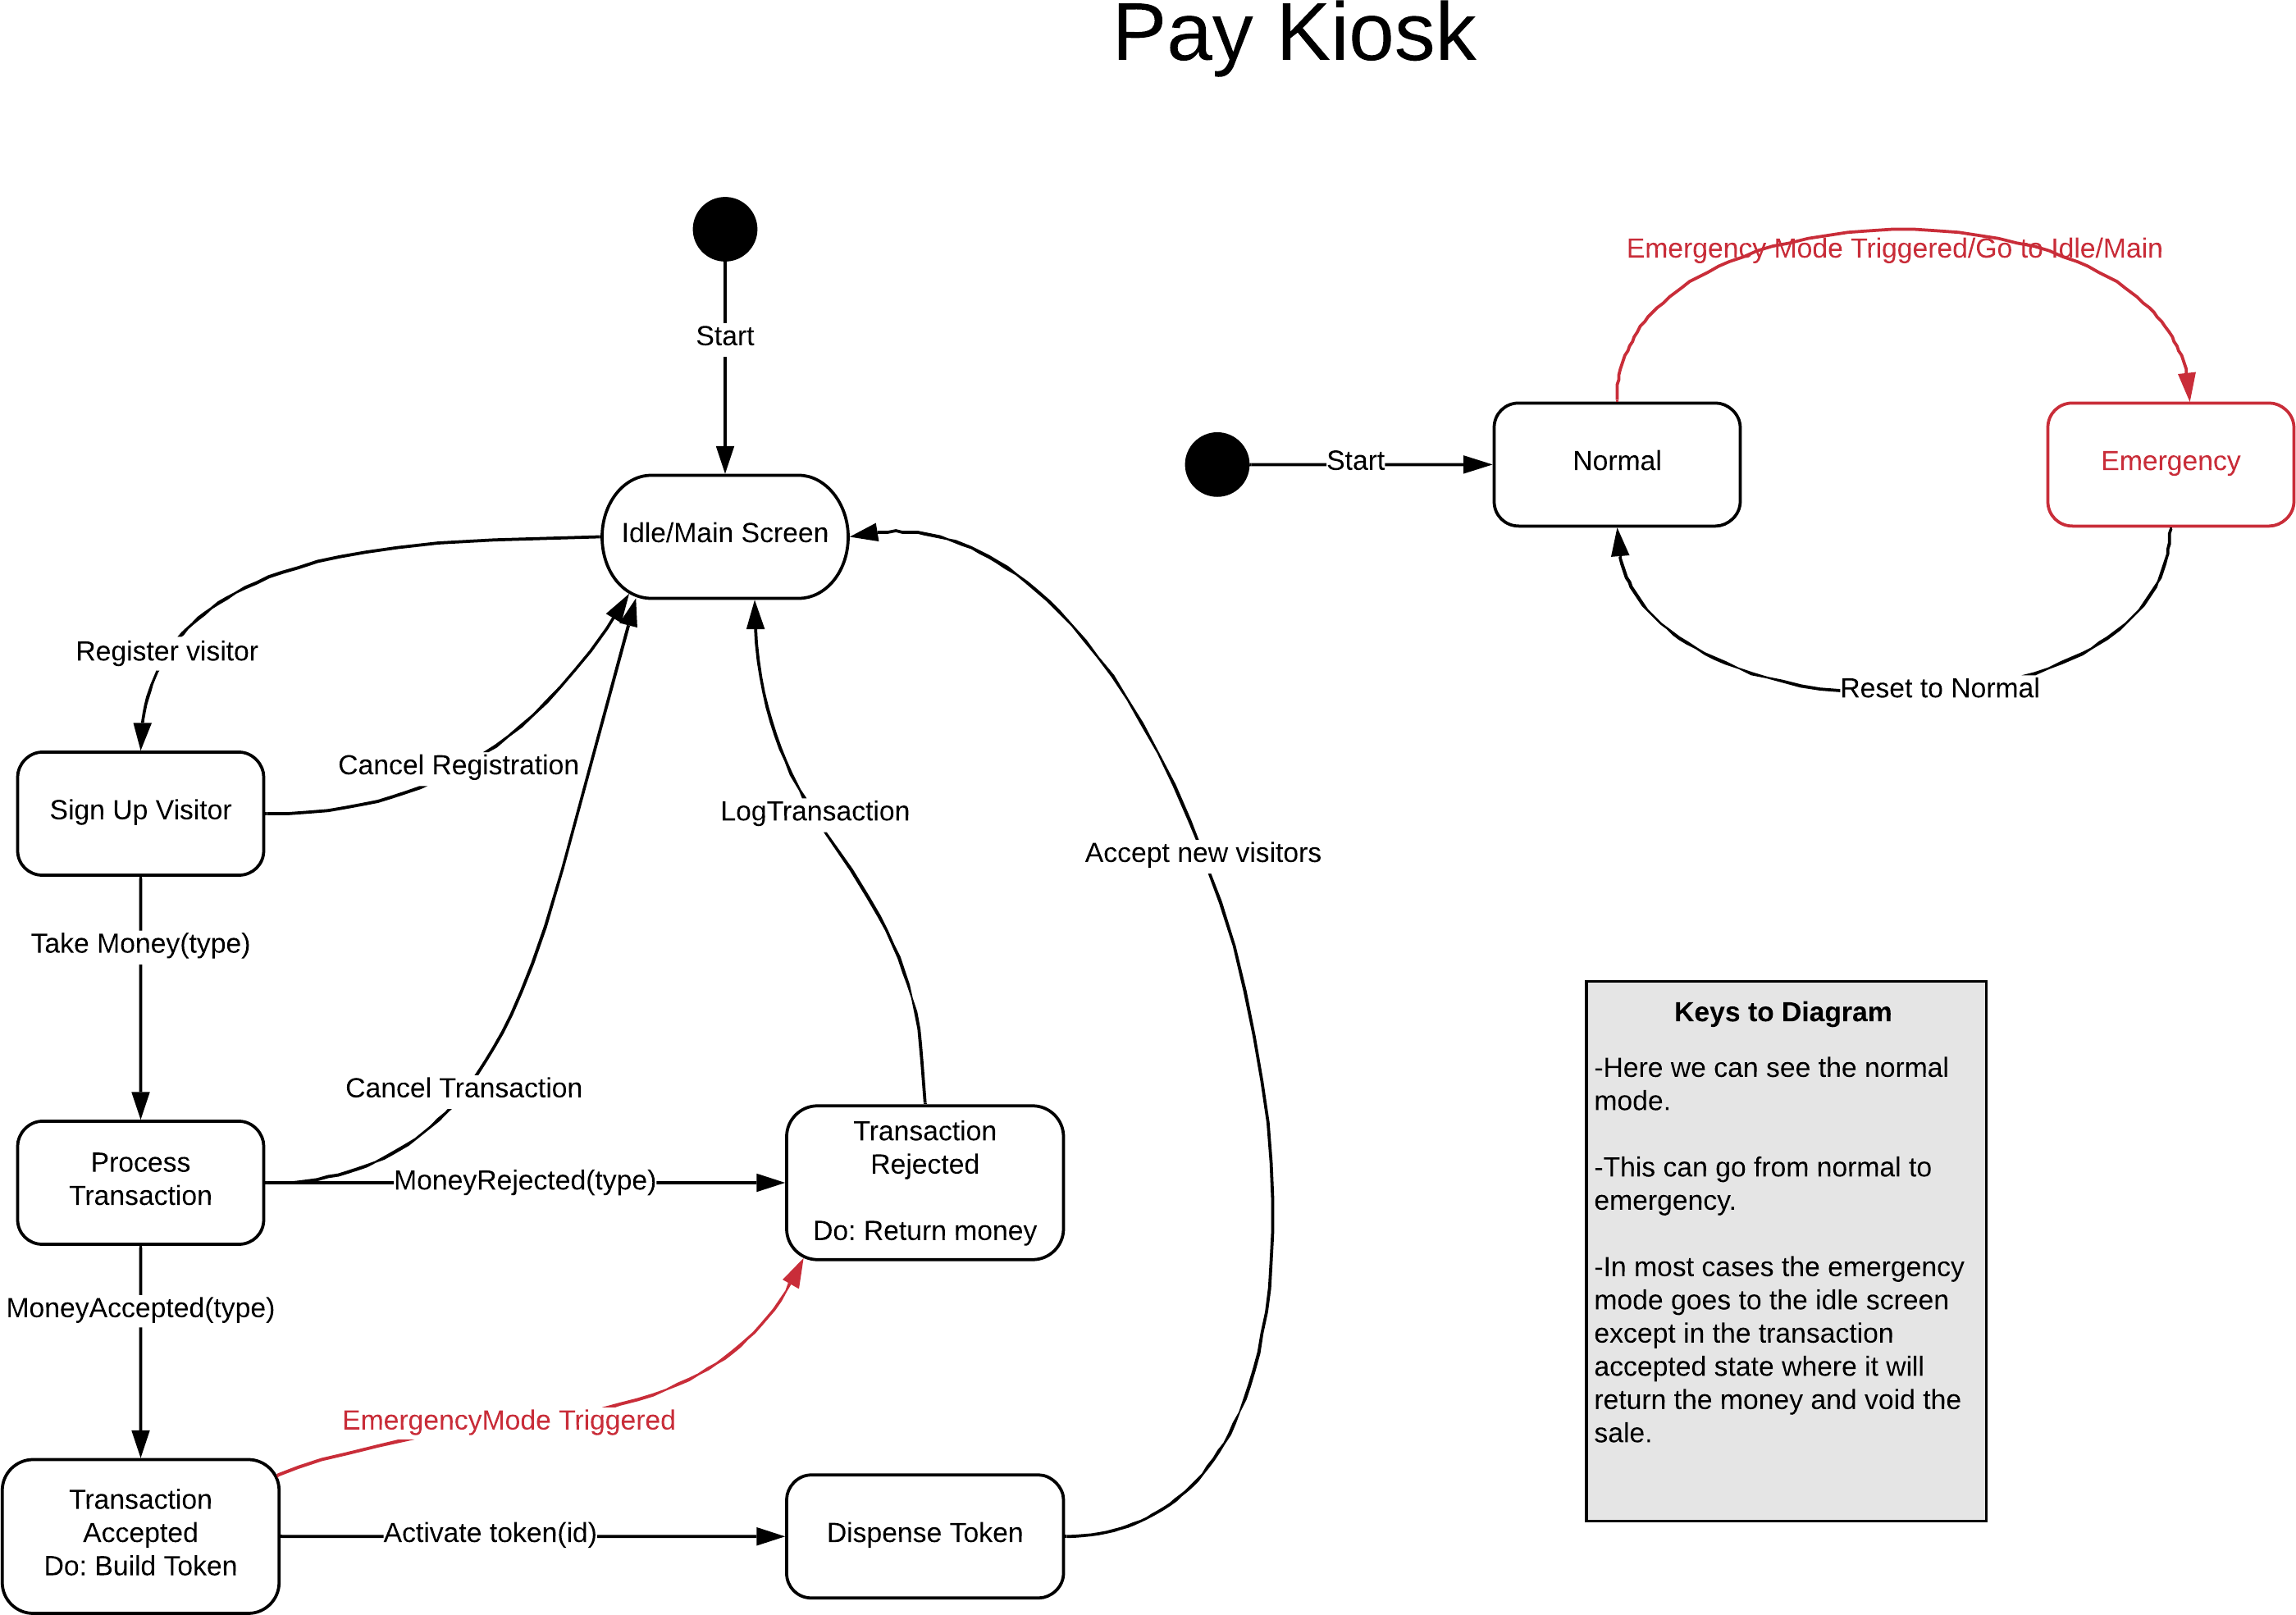
\includegraphics[scale=0.30]{PayKiosk.png}}
         \caption{Pay Kiosk Dynamic Control Model}
          \label{fig:paykiosk}
    \end{figure}

    \begin{figure}[H]
         {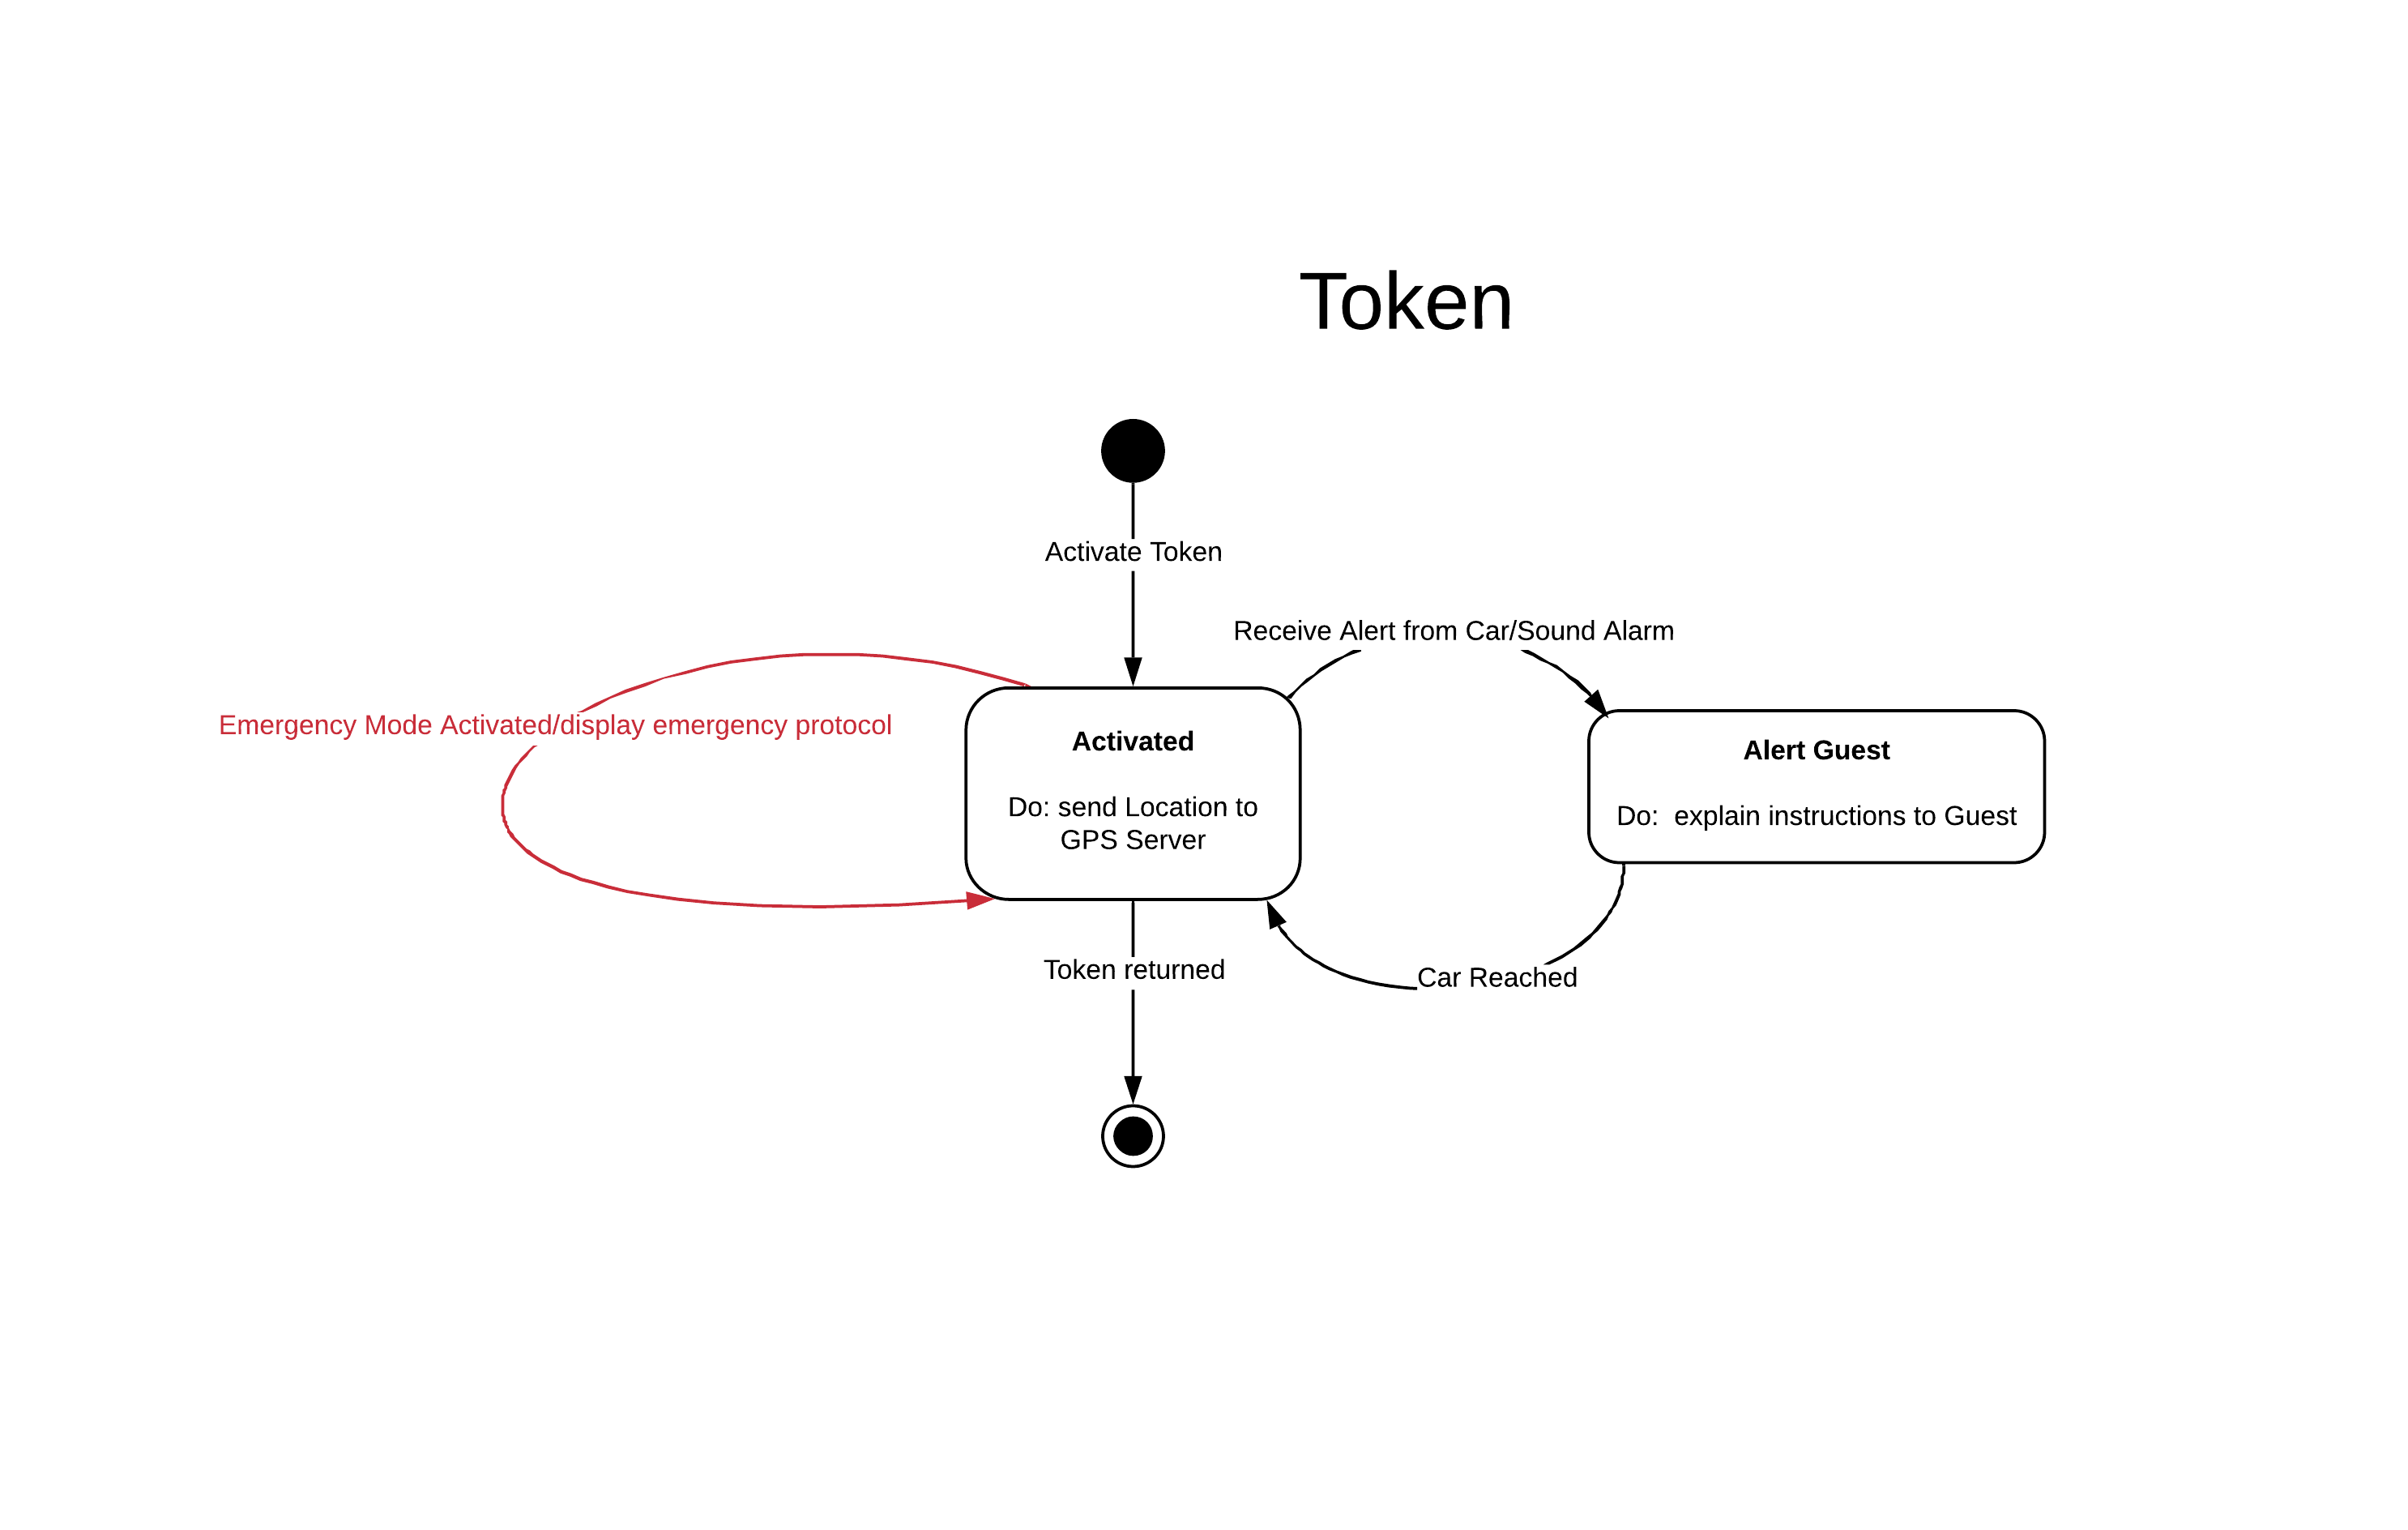
\includegraphics[scale=0.30]{Token.png}}
         \caption{Token Dynamic Control Model}
          \label{fig:token}
    \end{figure}

    \begin{figure}[H]
         \centerline{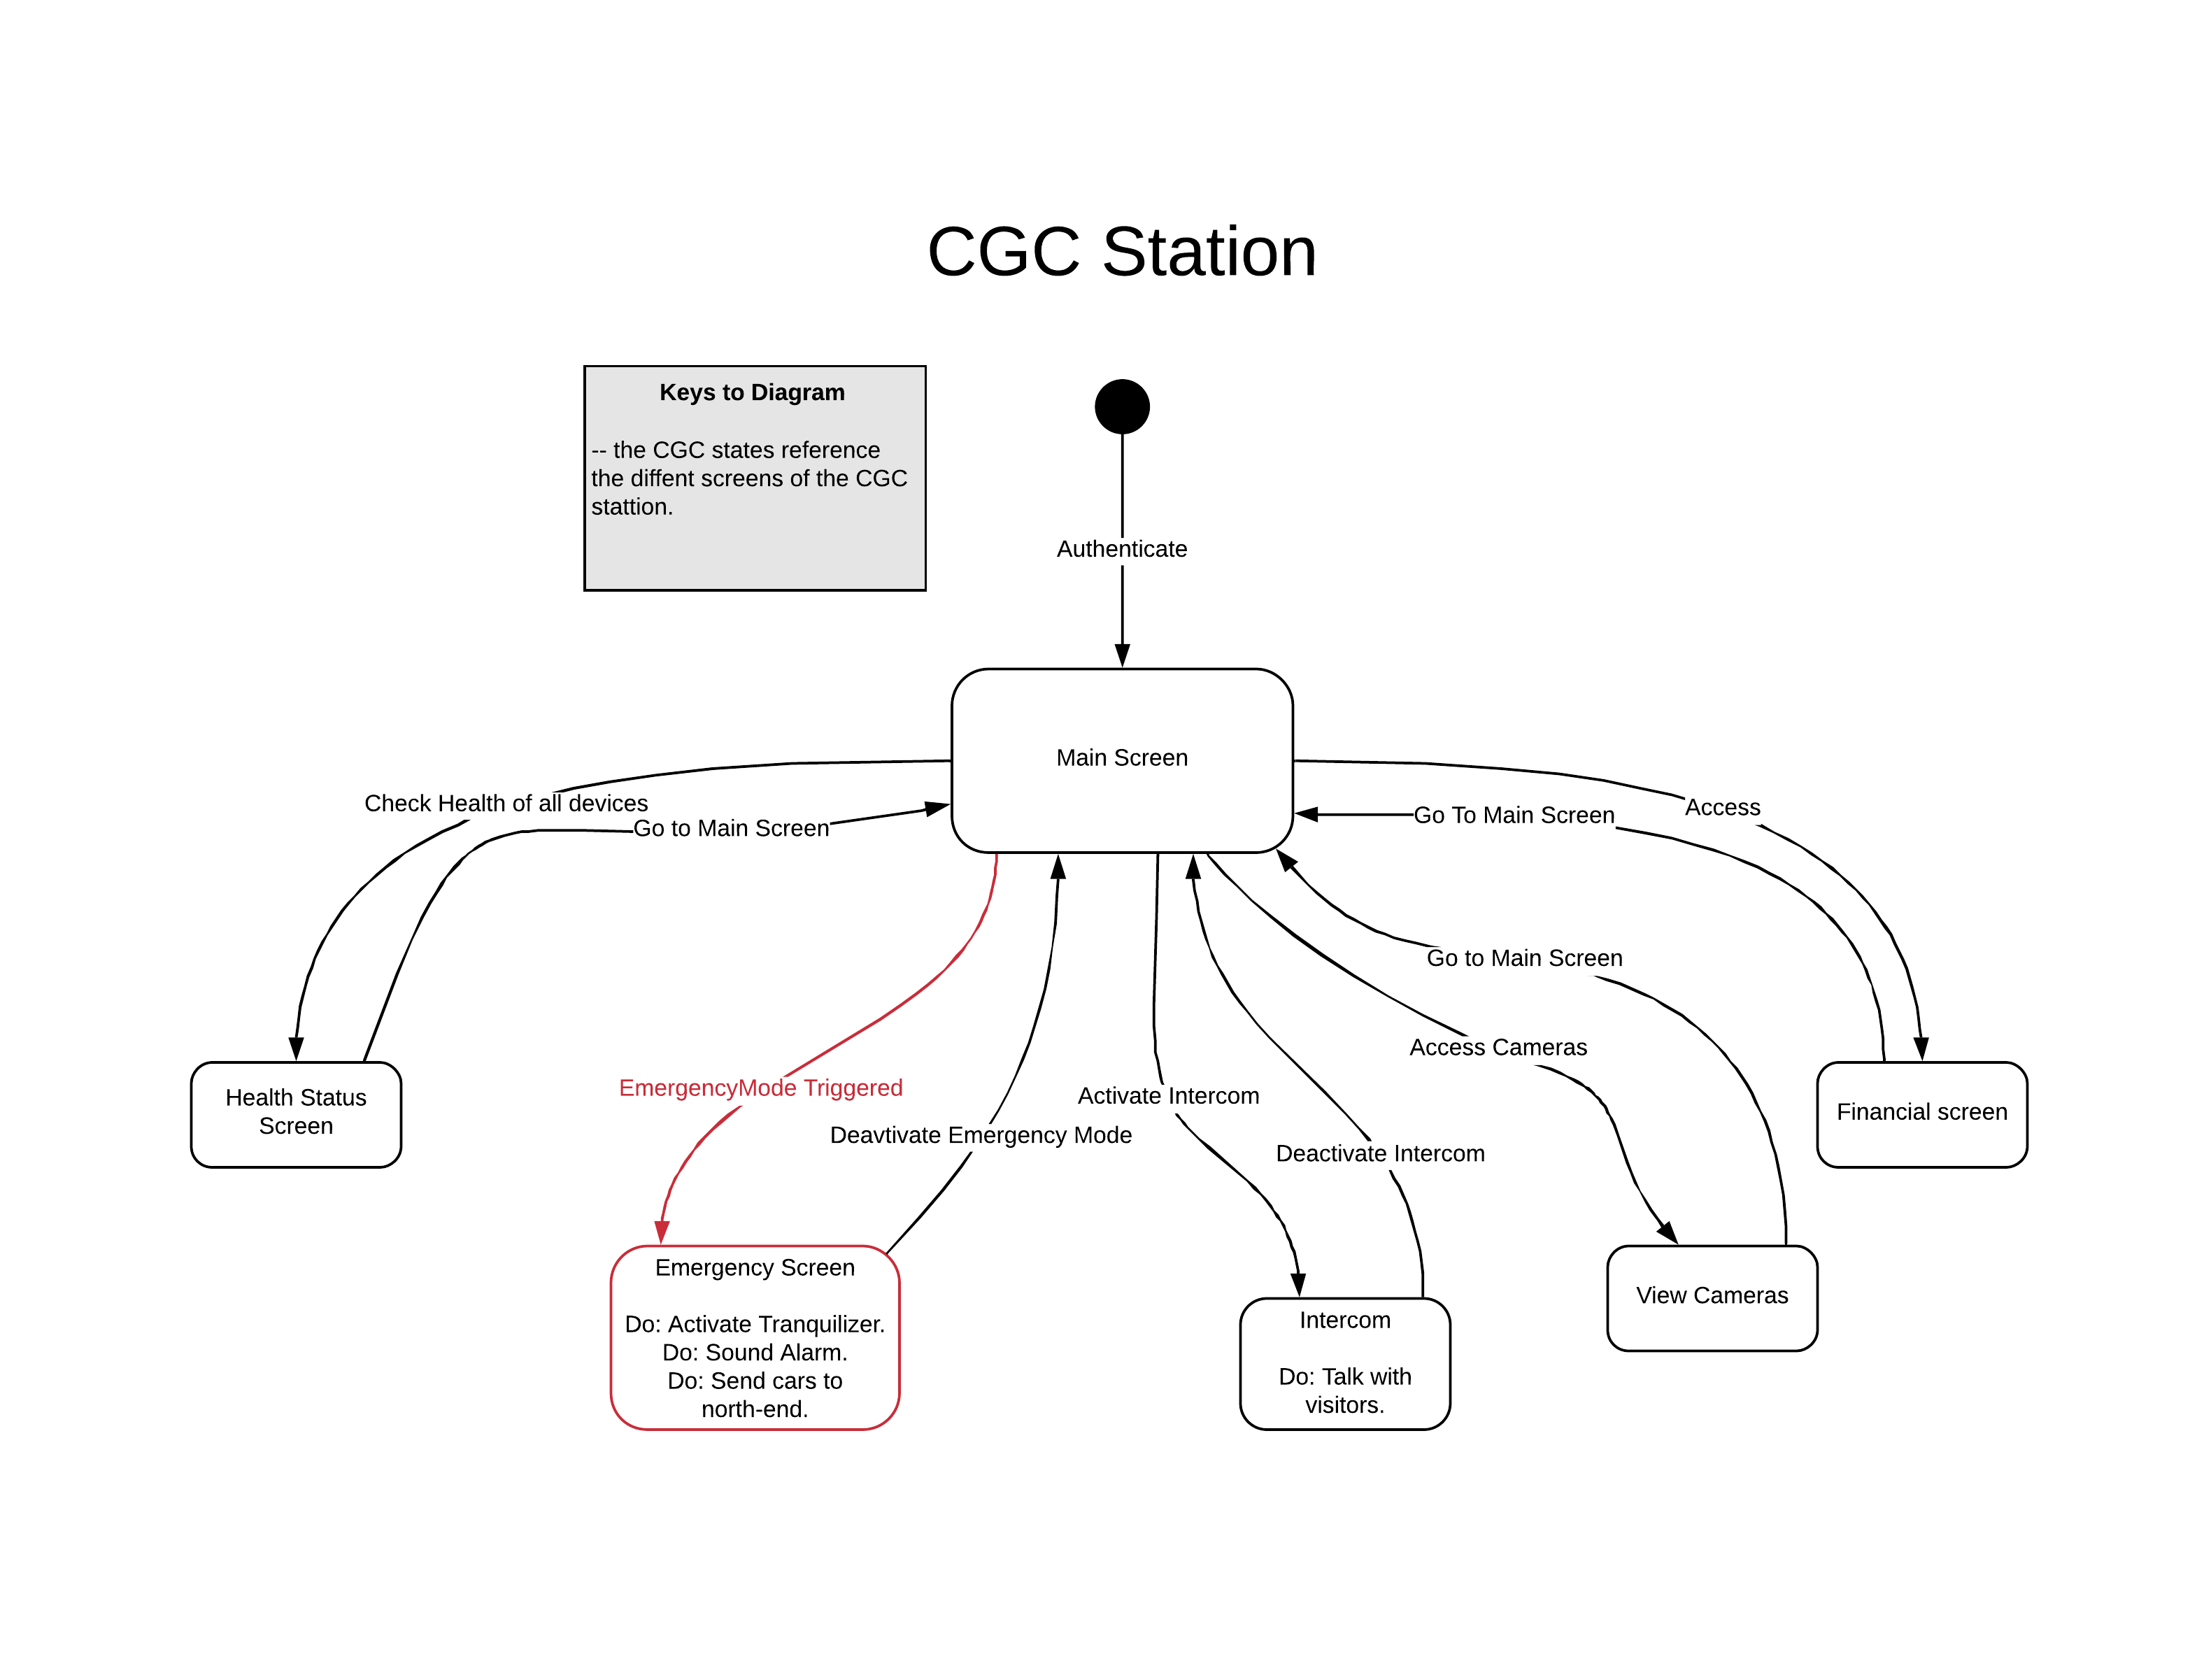
\includegraphics[scale=0.20]{CGCStation.png}}
         \caption{CGC Station Dynamic Control Model}
          \label{fig:cgcstation}
    \end{figure}

    \begin{figure}[H]
         \centerline{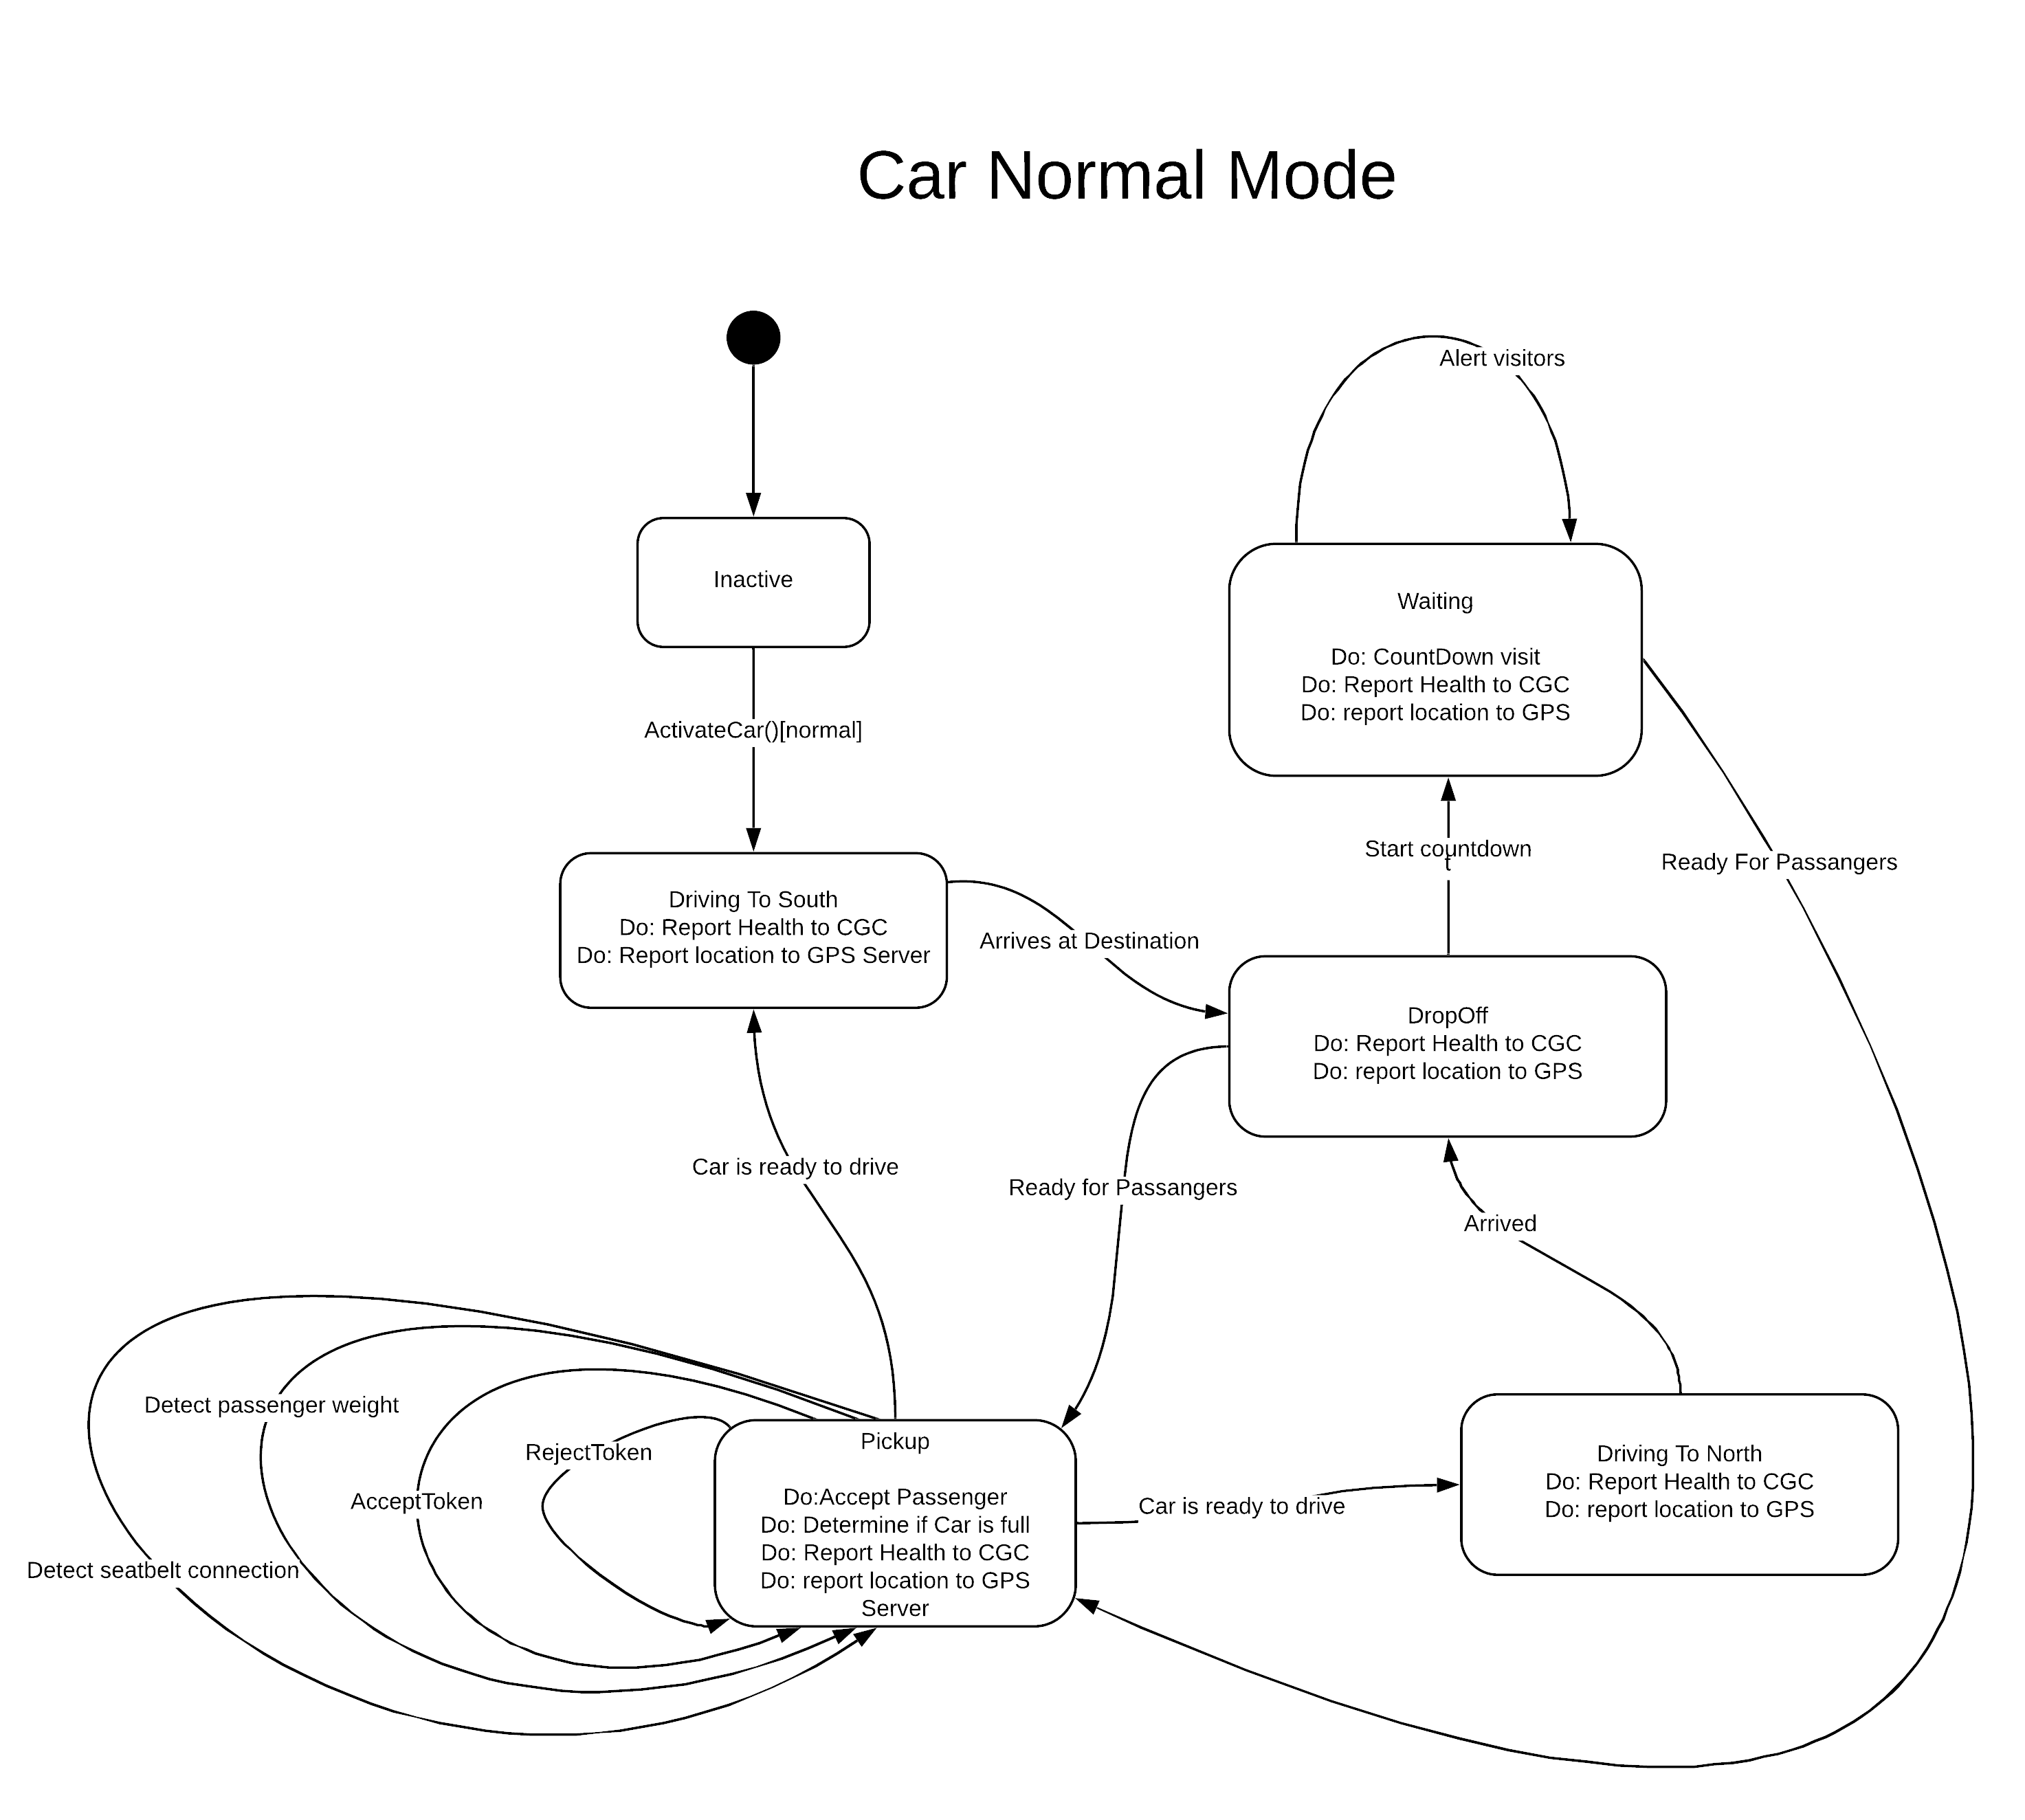
\includegraphics[scale=0.18]{CarNormalMode.png}}
         \caption{Car Normal Mode Dynamic Control Model}
          \label{fig:carnormalmode}
    \end{figure}

    \begin{figure}[H]
         \centerline{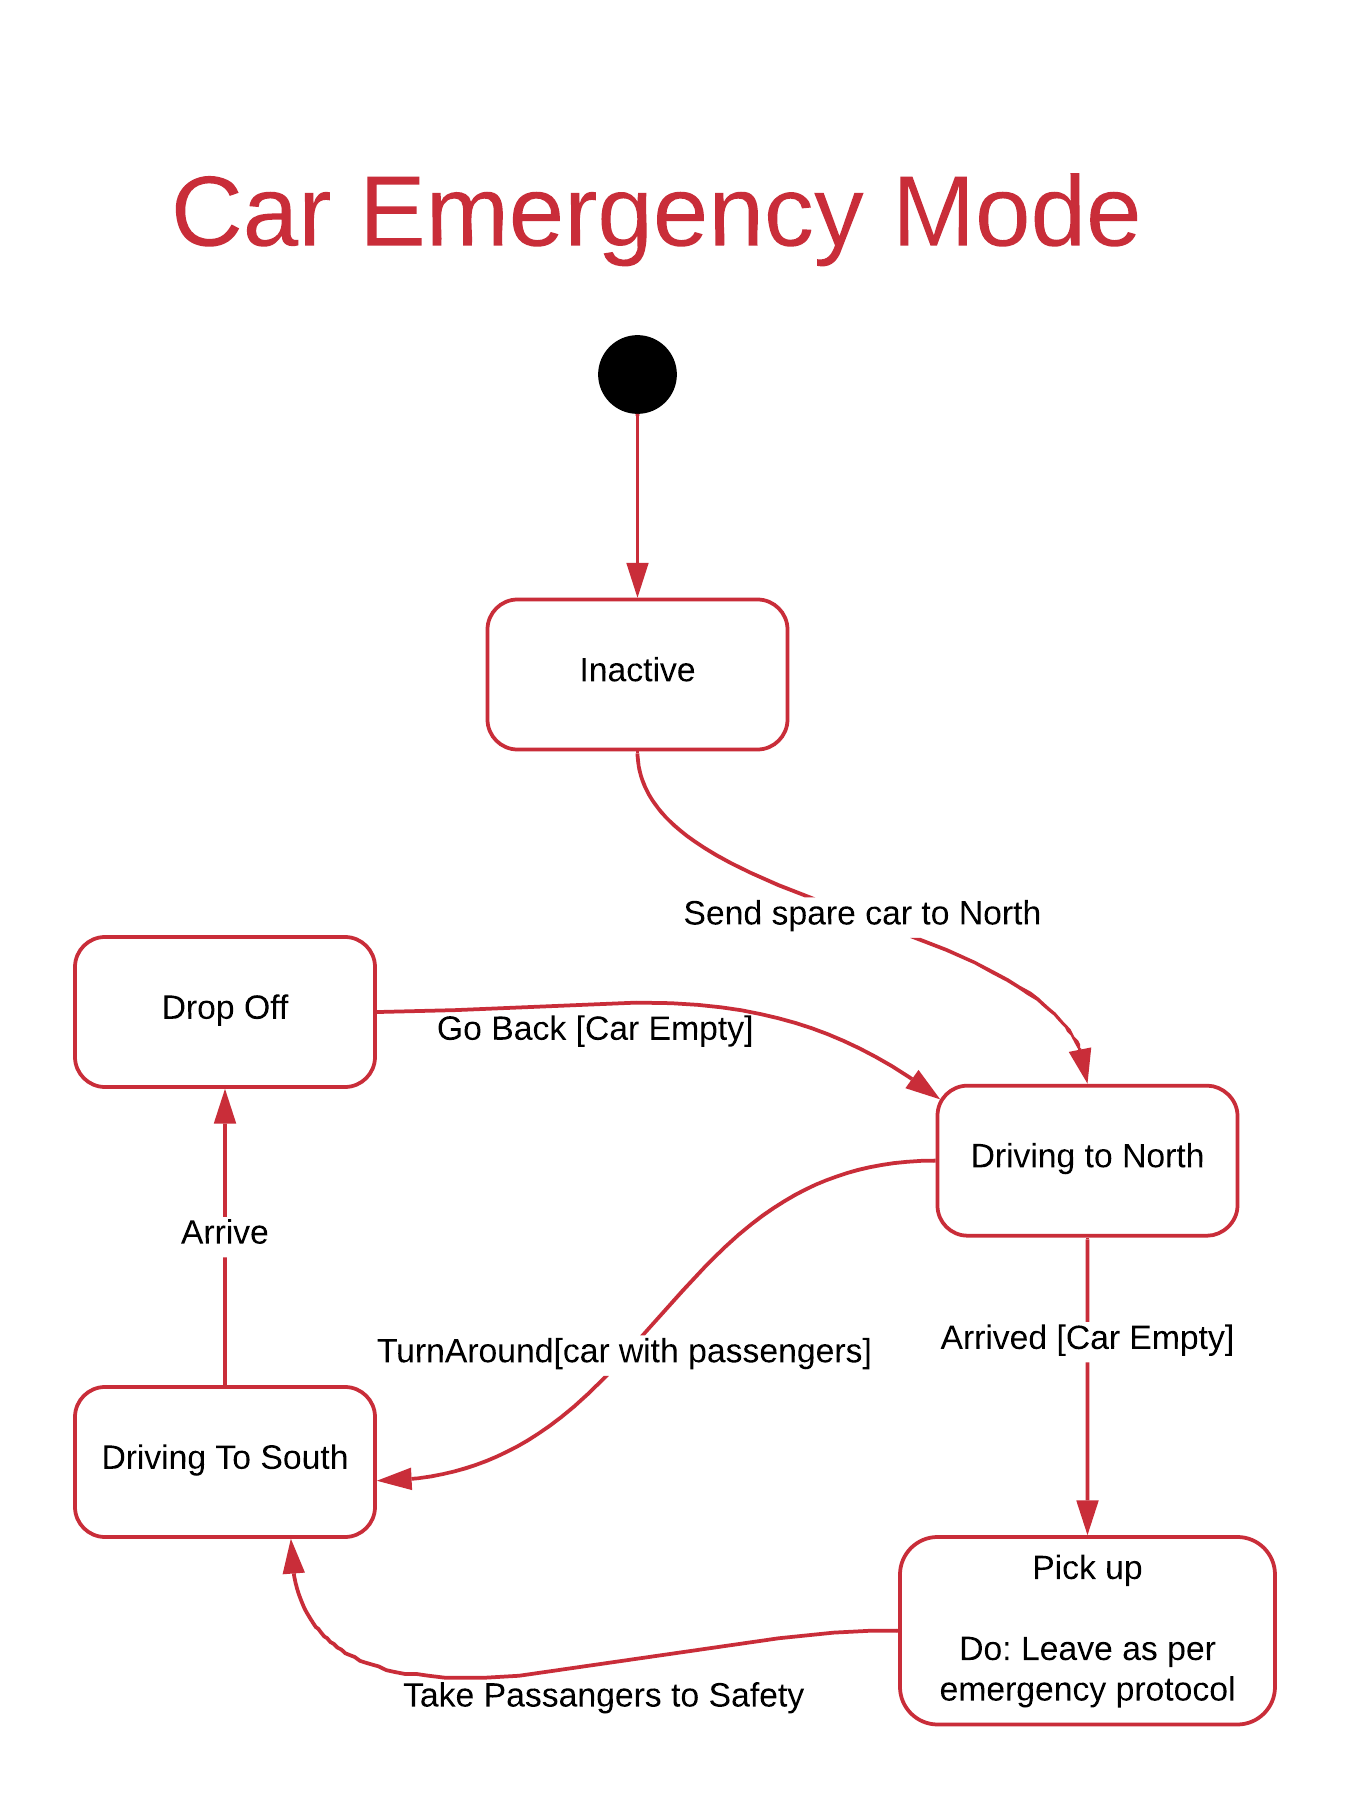
\includegraphics[scale=0.25]{CarEmergencyMode.png}}
         \caption{Car Emergency Mode Dynamic Control Model}
          \label{fig:caremergencymode}
    \end{figure}

    \begin{figure}[H]
         \centerline{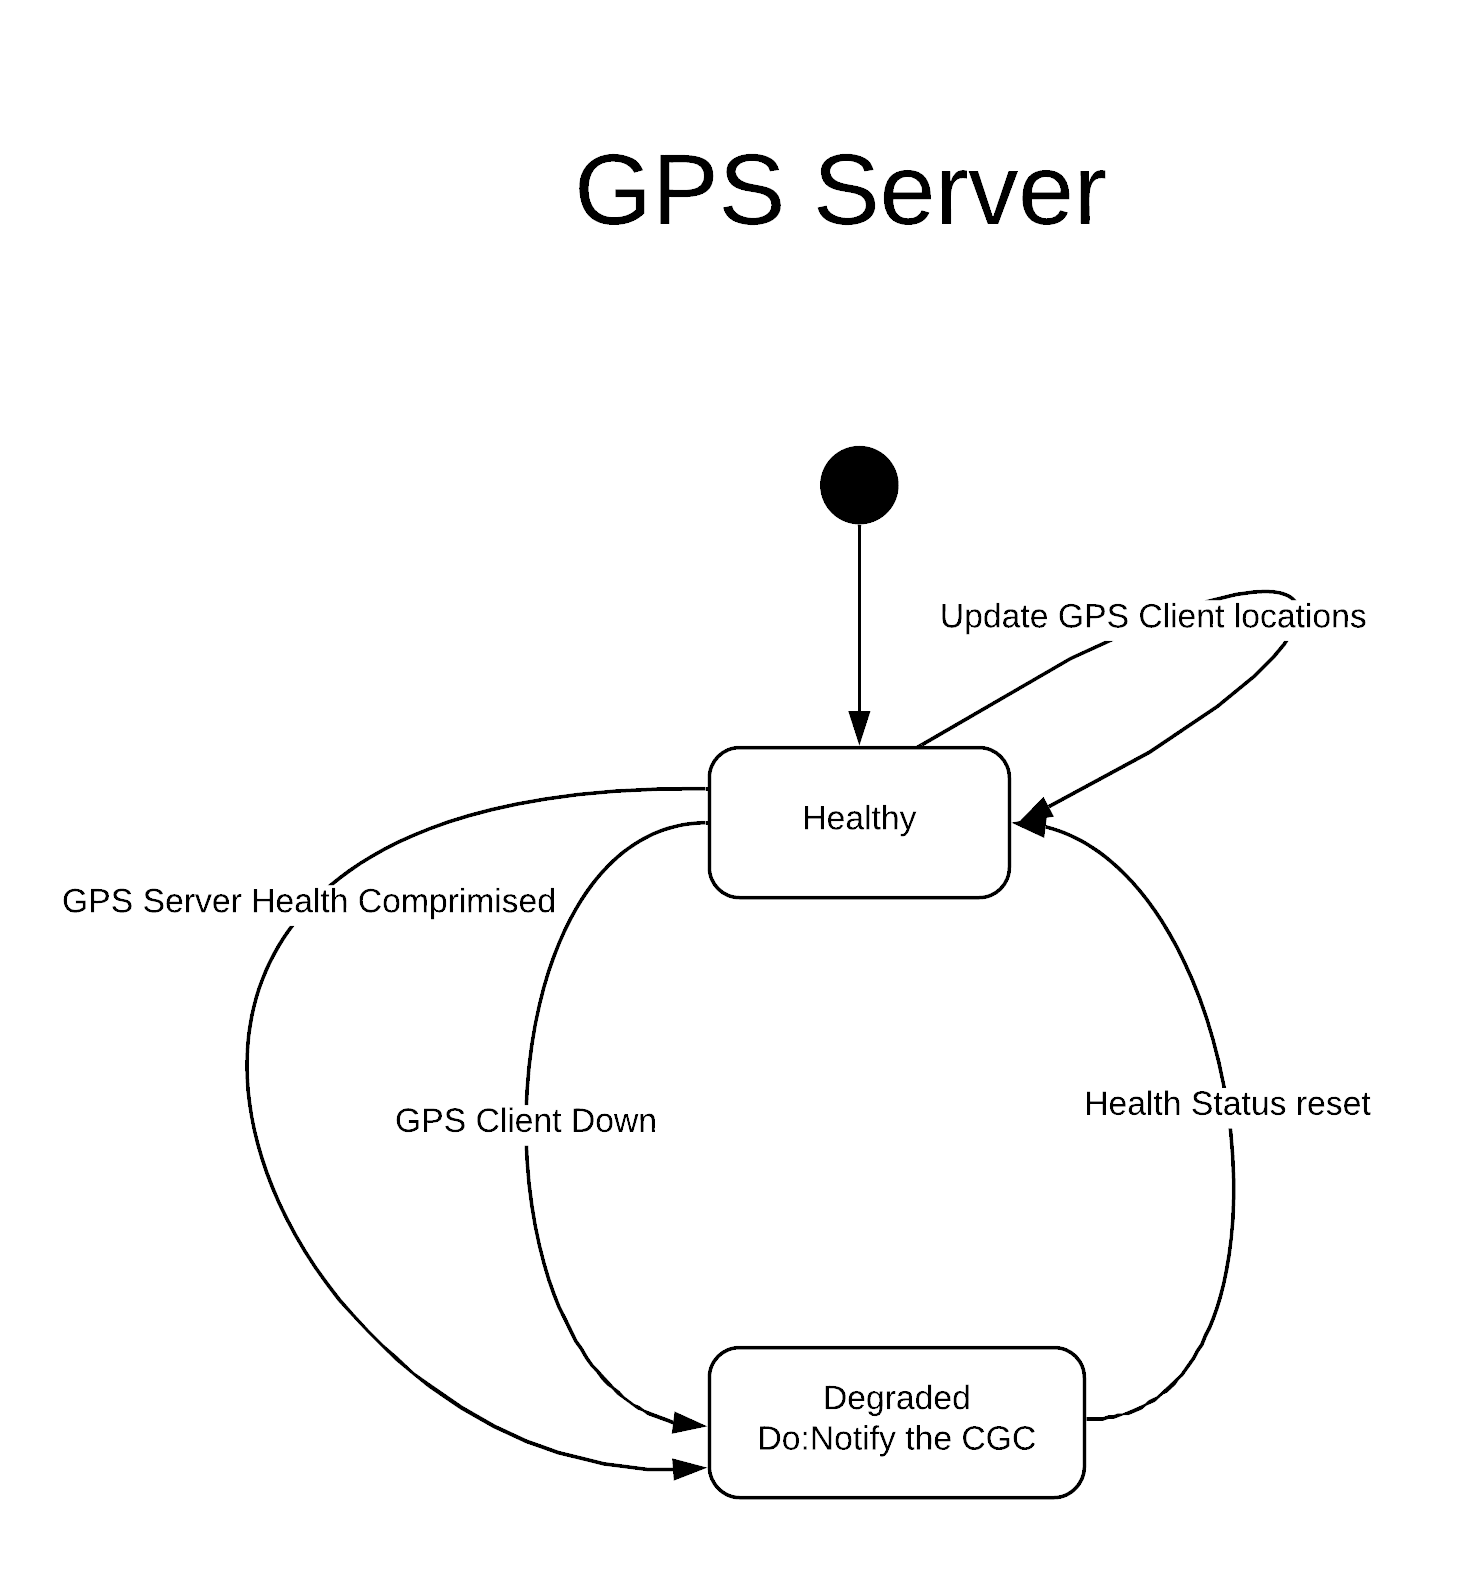
\includegraphics[scale=0.25]{GPSServer.png}}
         \caption{GPS Server Dynamic Control Model}
          \label{fig:gpsserver}
    \end{figure}

    \begin{figure}[H]
         \centerline{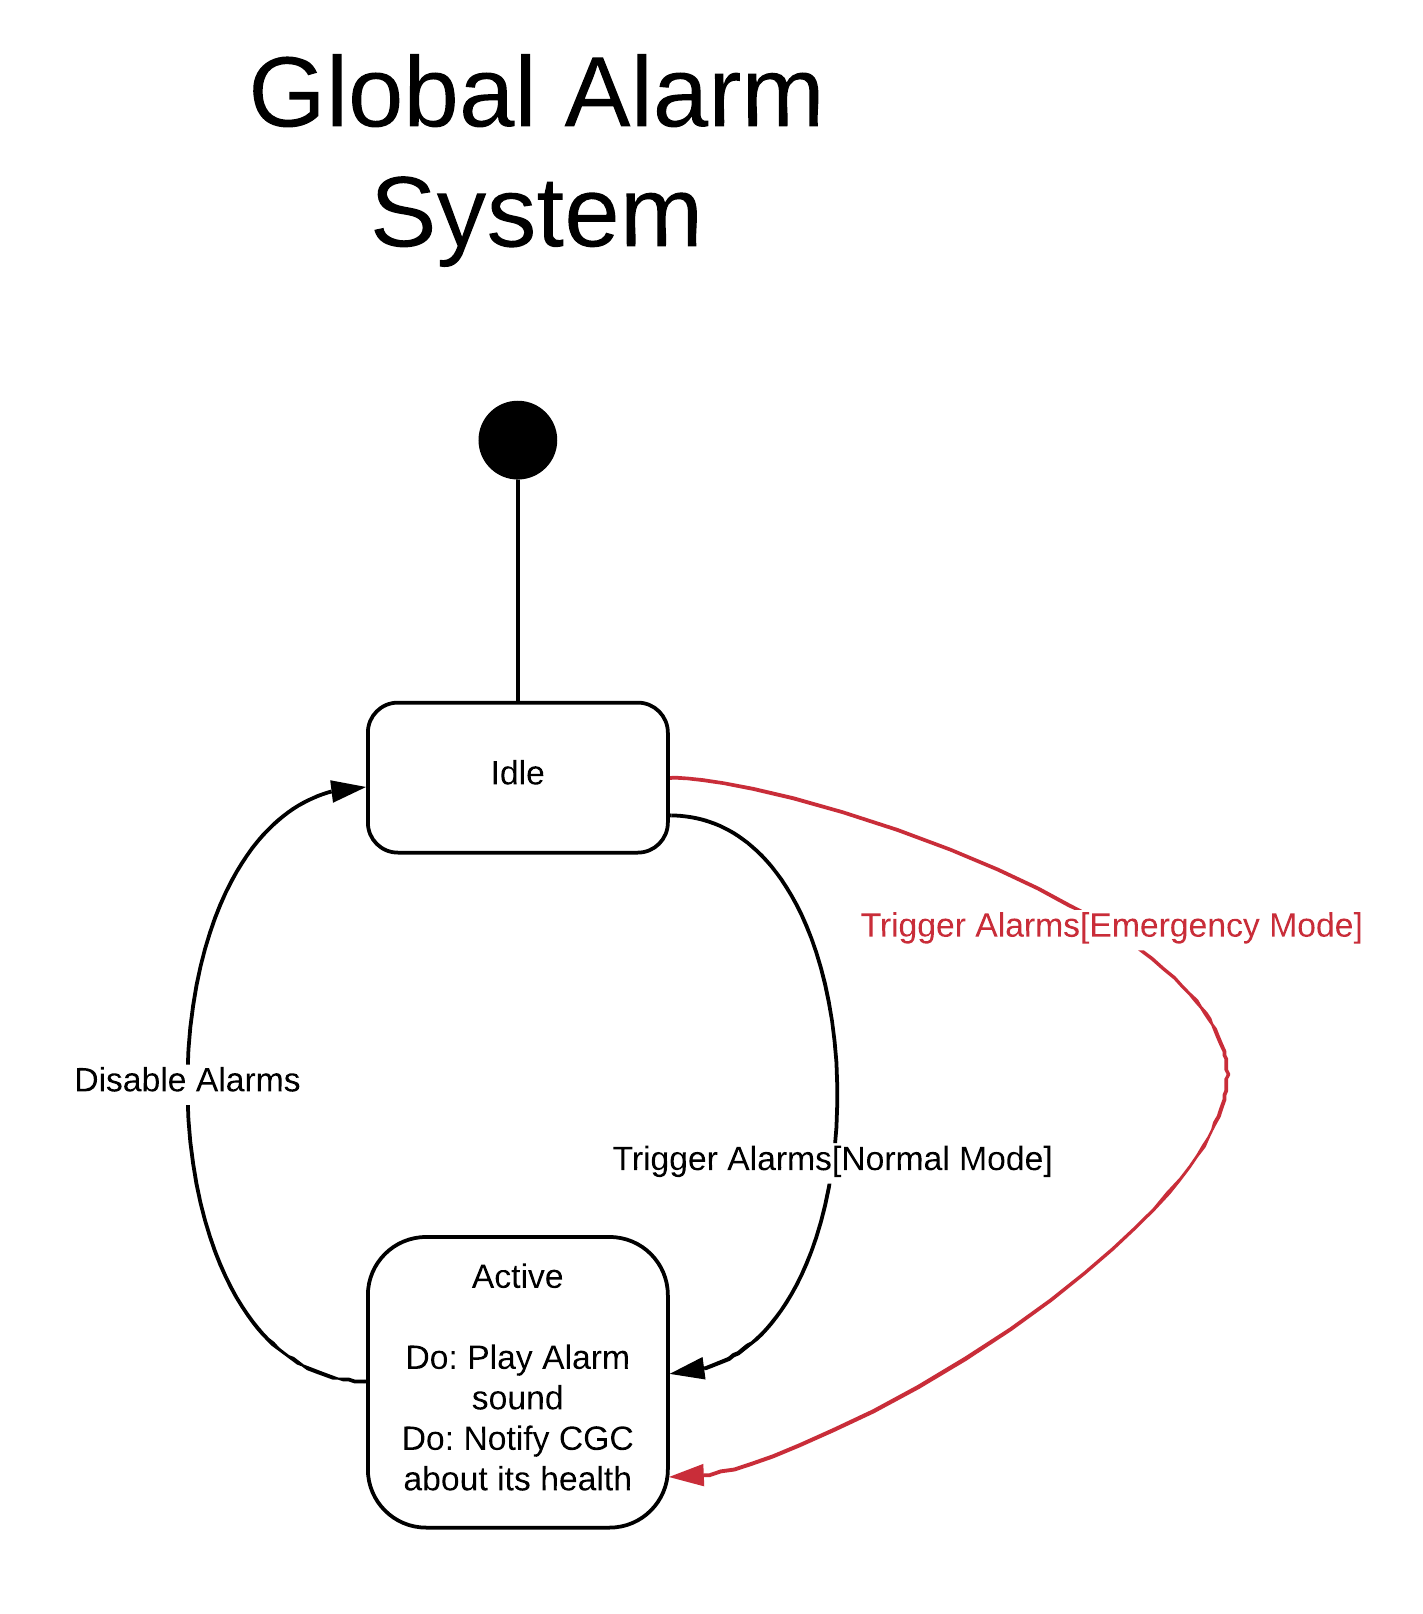
\includegraphics[scale=0.30]{GlobalAlarmSystem.png}}
         \caption{Global Alarm System Dynamic Control Model}
          \label{fig:globalalarmsystem}
    \end{figure}

    \begin{figure}[H]
         \centerline{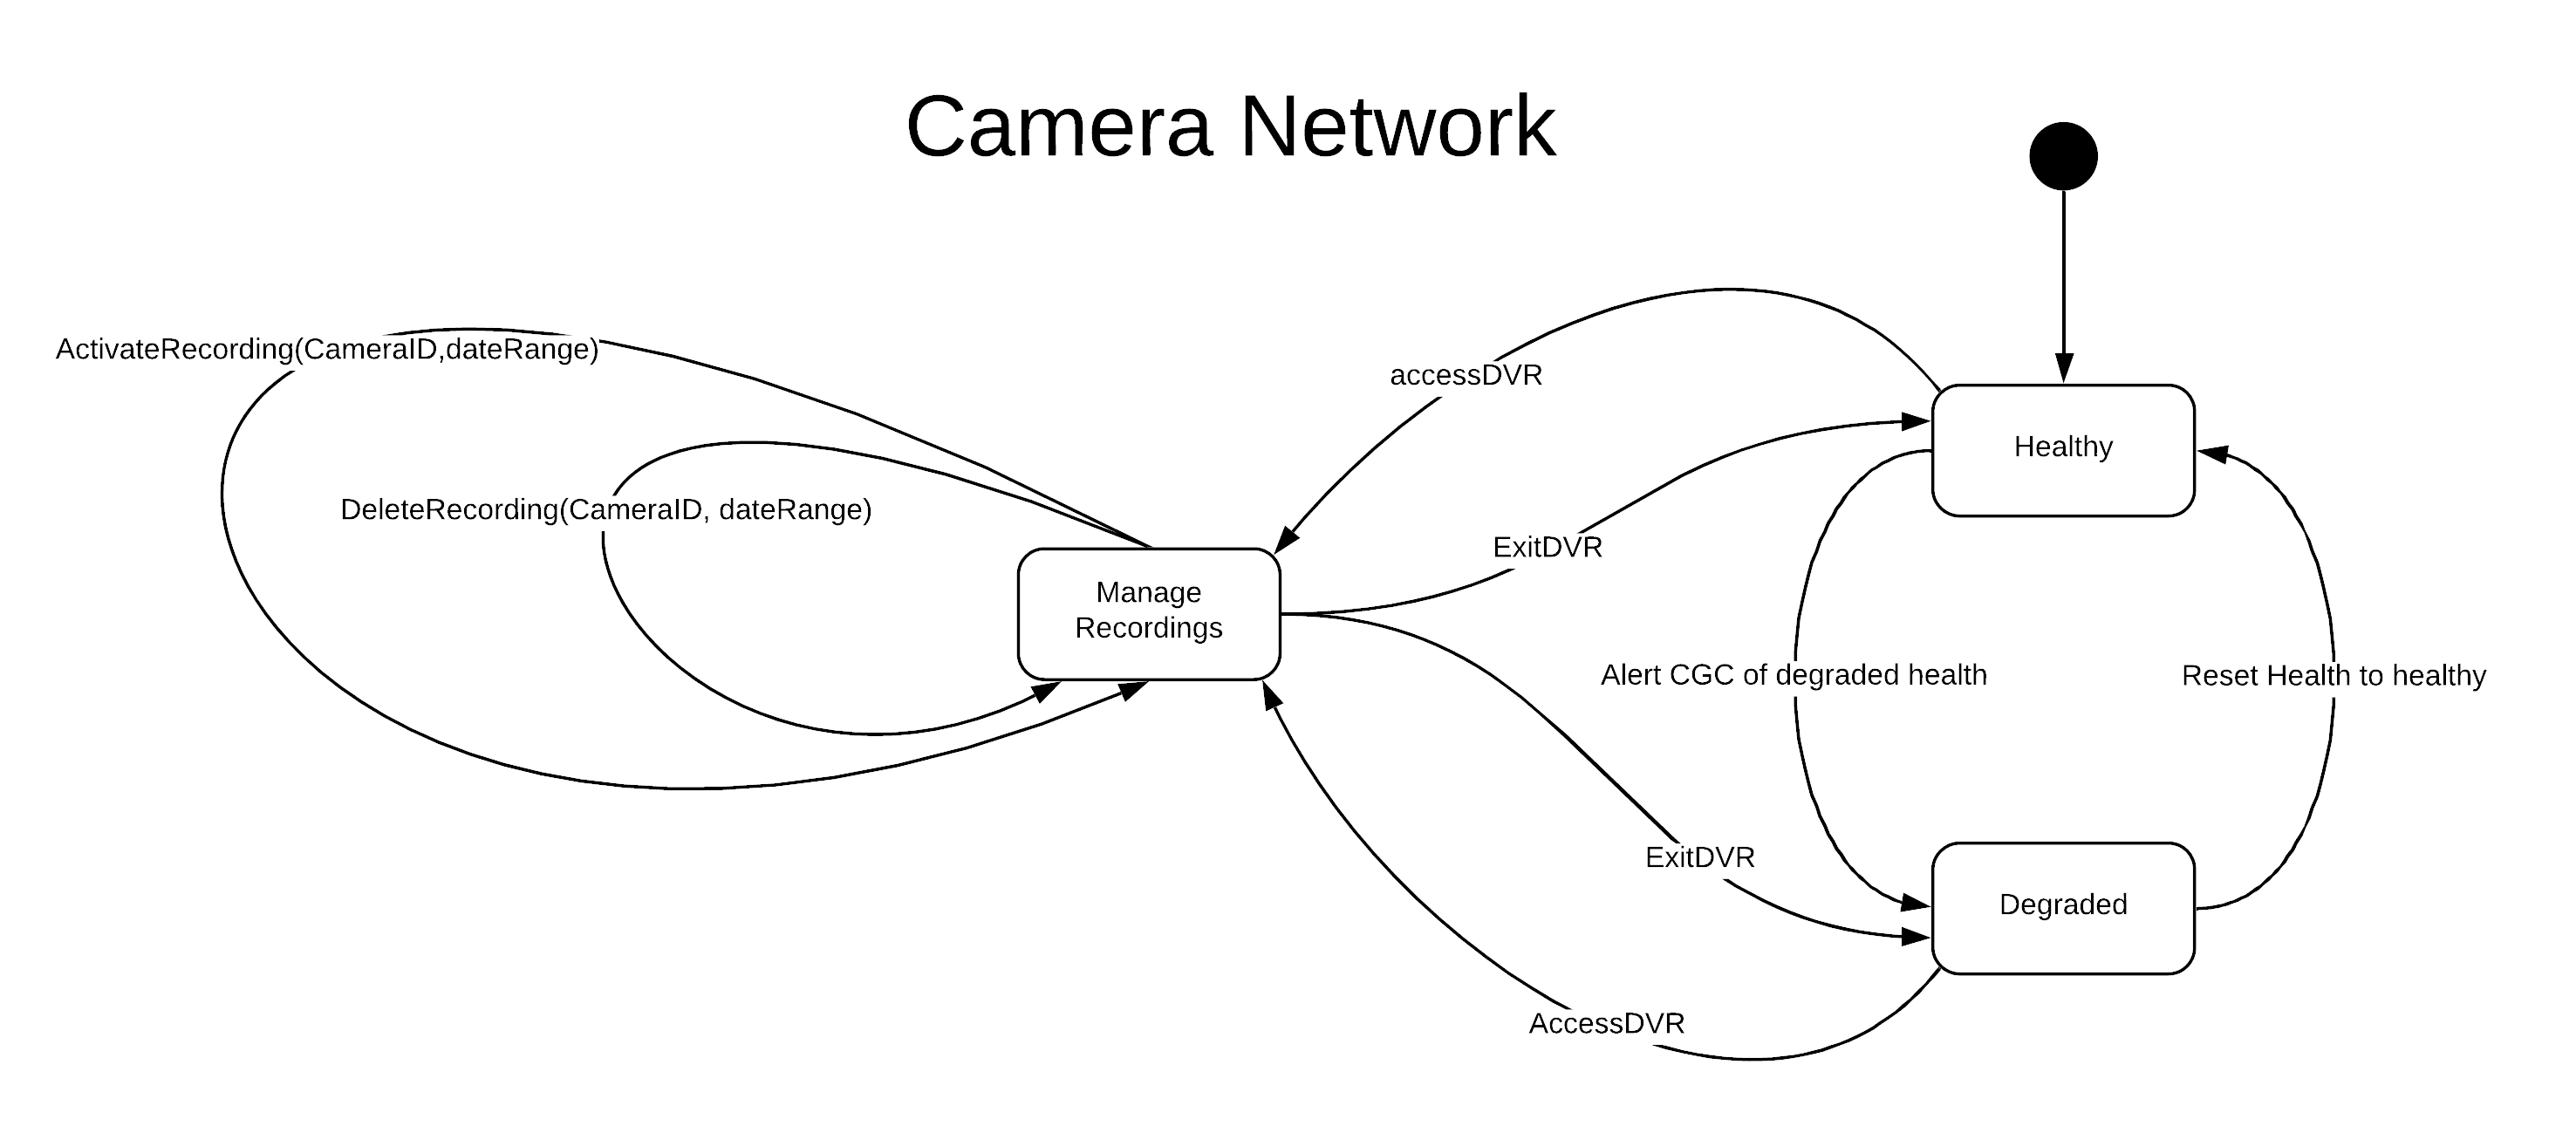
\includegraphics[scale=0.17]{CameraNetwork.png}}
         \caption{Camera Network System Dynamic Control Model}
          \label{fig:cameranetwork}
    \end{figure}

    \begin{figure}[H]
         \centerline{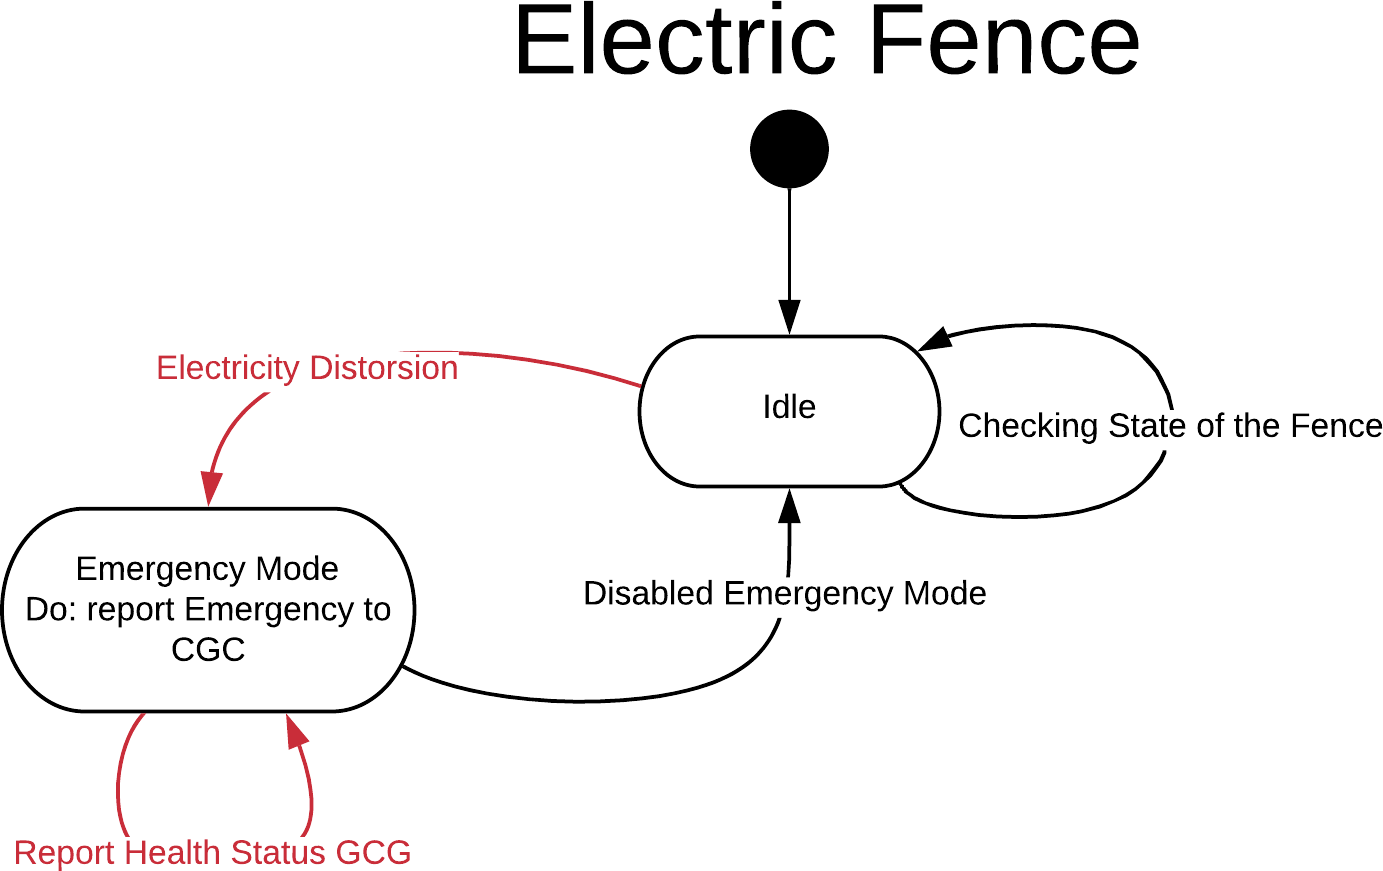
\includegraphics[scale=0.25]{ElectricFence.png}}
         \caption{Electric Fence Dynamic Control Model}
          \label{fig:electricfence}
    \end{figure}

    \begin{figure}[H]
         \centerline{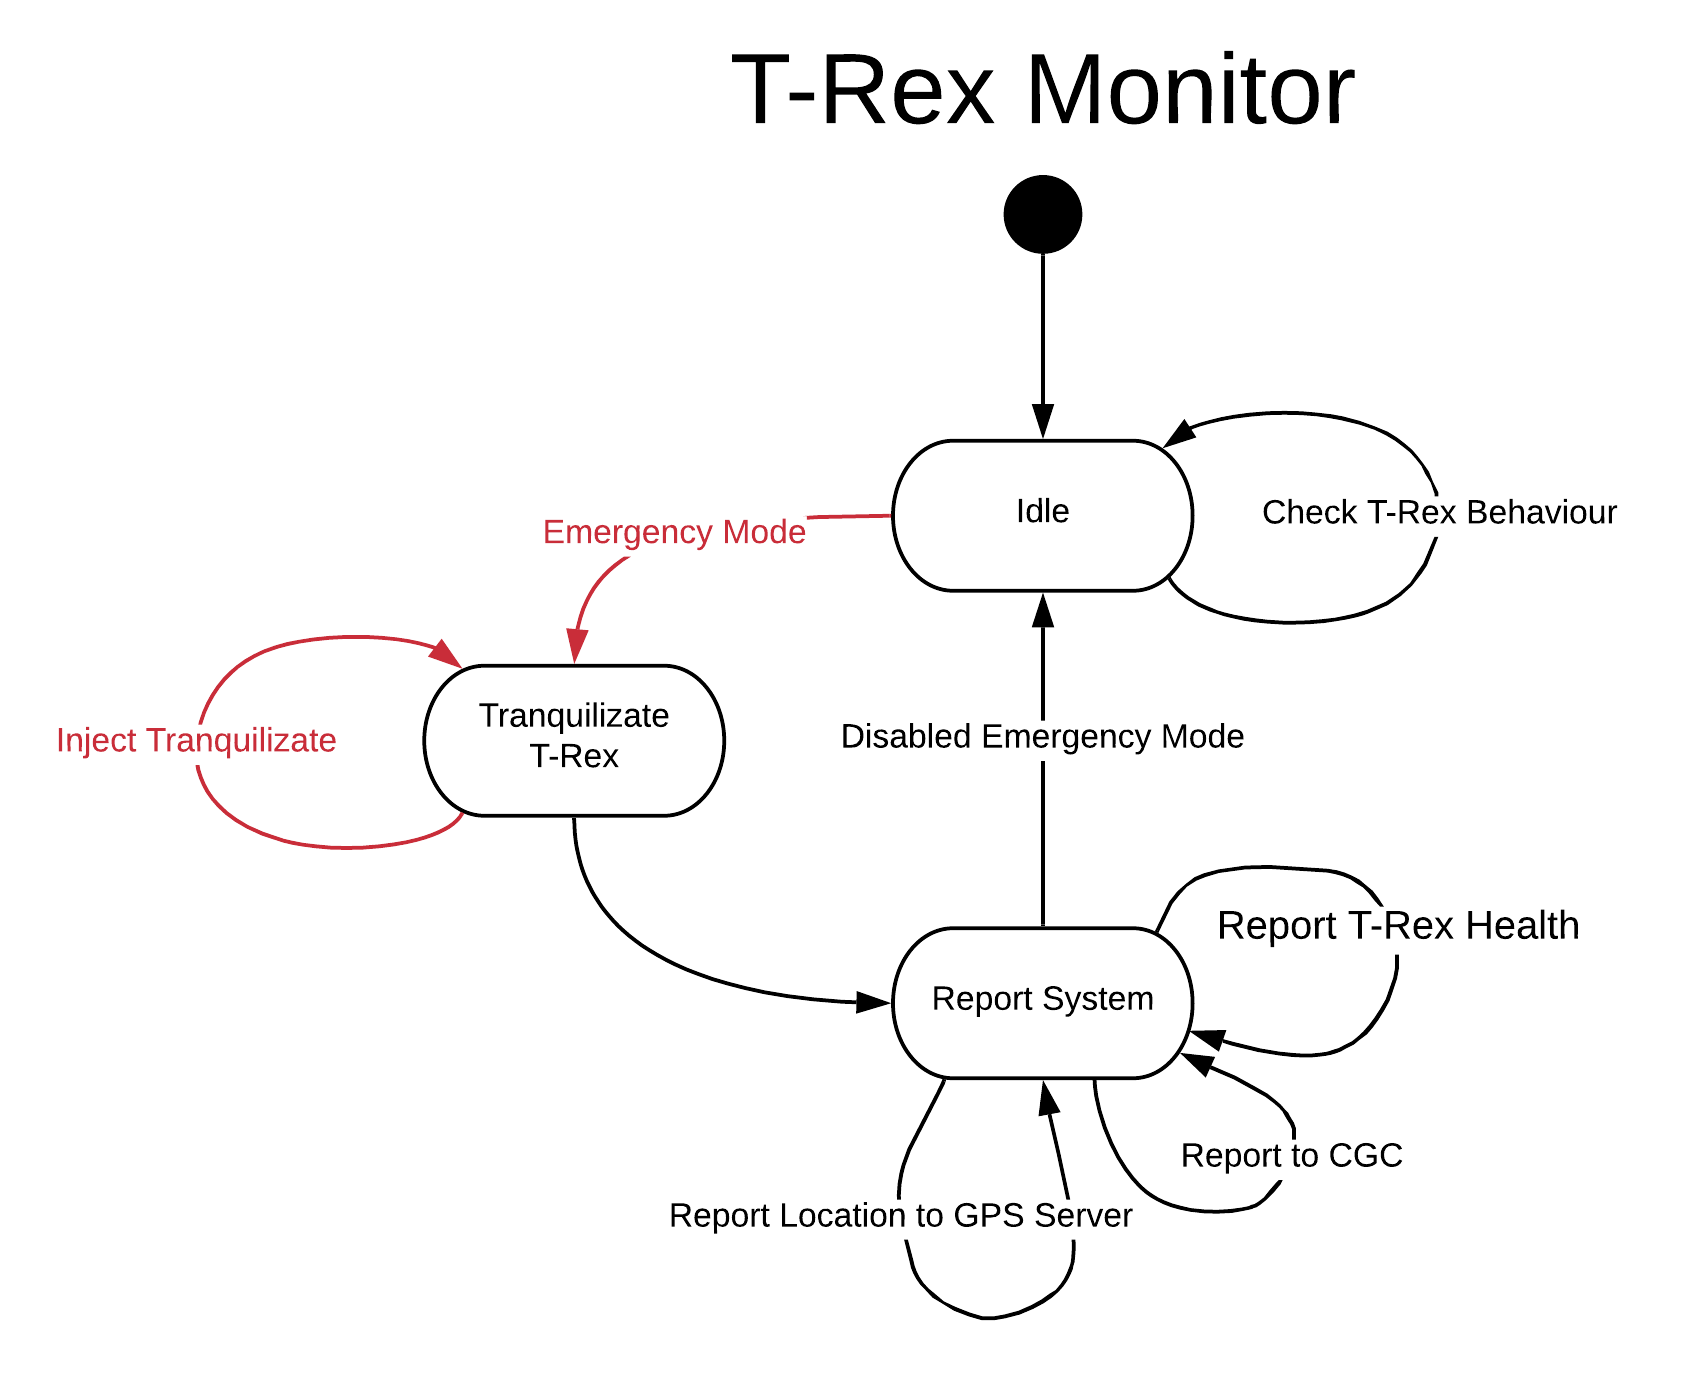
\includegraphics[scale=0.25]{T-RexMonitor.png}}
         \caption{T-Rex Monitor Dynamic Control Model}
          \label{fig:trexmonitor}
    \end{figure}

\section{Design Constraints} \label{cons} %
% error handling, exceptions, hazards, 
\paragraph{} \textit{There are quite a bit of constraints\footnote{Design Constraints by Anas Gauba} that the CGC must address in order to successfully function.}

    \subsection{Client}
    \begin{itemize}
        \item The visitors must arrive and purchase tokens from the pay kiosks on the south-end of the island. 
        \item The visitors must get a token which acts as a GPS device as well as RFID key to easily access the perks. 
        \item There must only be one token per visitor.
    \end{itemize}

    \subsection{Safety}
    \begin{itemize}
        \item There must be an emergency mode in the event of the enclosure failure.
        \item The vehicles must alert and instruct visitors in the event of an emergency.
        \item The alarm system must be audible on both the north and south ends.
        \item The vehicles must facilitate evacuation in the event of an emergency.
        \item There must be a surplus of vehicles on either end of the island at all times.
        \item The tokens must provide additional evacuation information such as visitor's location.
        \item The cars must maintain safe speeds at all times.
        \item The cars must lock the doors before moving to its destination.
    \end{itemize}

    \subsection{Regulations}
    \begin{itemize}
        \item The vehicles should accommodate up to ten visitors (excluding the emergency scenario).
        \item The vehicles must alert visitors once their allotted time is up. 
    \end{itemize}

    \subsection{Security}
    \begin{itemize}
        \item The T-Rex location is critical and it must be known at all times.
        \item The camera network stream must be available around the island at all times.
        \item The employee must directly monitor the health of all the devices, especially the ones which can cause harm to the visitors, such as, T-Rex and Electric Fence. 
    \end{itemize}

\section{Sample Use Cases}
\paragraph{} \textit{The CGC lends itself for a substantial amount of uses. Some notable uses include financial,
official, managerial, medical, and technical connotations.}

%%%%%% Anas %%%%%
%    \subsection{Bookkeeper}
%    \textit{brief description of actor}
%    \par\noindent\rule{\textwidth}{0.4pt}    
%    \begin{itemize}
%        \item[]\textbf{Use Case:}                                
%            *DoSomething (the name of the action to be executed by actor)*
%
%        \item[]\textbf{Primary Actor:}
%            *ThatWhichWishesToDoSomething (name of actor)*
%
%        \item[]\textbf{Goal in Context:}
%            *that which is to be accomplished by the action*
%
%        \item[]\textbf{Preconditions:}
%            *states of the actor and system prior to the action*
%
%        \item[]\textbf{Trigger:}
%            *that which initiates the action (e.g. actor breaks out of enclosure)*
%
%        \item[]\textbf{Scenario:}
%            *sequence of actions from trigger to goal*
%            \begin{enumerate}
%                \item first event
%                \item second event
%                \item ...
%            \end{enumerate}
%
%        \item[]\textbf{Exceptions:}
%            *edge cases, potential hazards, errors, etc*
%            \begin{itemize}
%                \item[] some exception
%                \item[] some other exception                
%                \item[] ...
%            \end{itemize}
%
%        \item[]\textbf{Priority:}
%            *level of implementation importance (e.g. correct change is a must)*
%
%        \item[]\textbf{When Available:}
%            *when or during which interval of time the action is to supported by the system*
%
%        \item[]\textbf{Frequency of Use:}
%            *number of uses per unit of time (e.g. annually, billions per second, etc)*
%
%        \item[]\textbf{Channel to Primary Actor:}
%            *means through which the system interacts with actor*
%
%        \item[]\textbf{Channels to Secondary Actors:}
%            *means through which the primary and secondary actors interact*
%            \begin{itemize}
%                \item[] some channel
%                \item[] some other channel
%                \item[] ...
%            \end{itemize}
%        \item[]\textbf{Secondary Actors:}
%            *intermediary or auxillary actors required to complete the goal*
%
%        \item[]\textbf{Open Issues:}
%            *itemization of current problems with any of the above*
%            \begin{itemize}
%                \item[] some issue
%                \item[] some other issue
%                \item[] ...
%            \end{itemize}
%    \end{itemize}
%    
%    \subsection{CGC Station Operator}
%    \textit{brief description of actor}
%    \par\noindent\rule{\textwidth}{0.4pt}    
%    \begin{itemize}
%        \item[]\textbf{Use Case:}                                
%            *DoSomething (the name of the action to be executed by actor)*
%
%        \item[]\textbf{Primary Actor:}
%            *ThatWhichWishesToDoSomething (name of actor)*
%
%        \item[]\textbf{Goal in Context:}
%            *that which is to be accomplished by the action*
%
%        \item[]\textbf{Preconditions:}
%            *states of the actor and system prior to the action*
%
%        \item[]\textbf{Trigger:}
%            *that which initiates the action (e.g. actor breaks out of enclosure)*
%
%        \item[]\textbf{Scenario:}
%            *sequence of actions from trigger to goal*
%            \begin{enumerate}
%                \item first event
%                \item second event
%                \item ...
%            \end{enumerate}
%
%        \item[]\textbf{Exceptions:}
%            *edge cases, potential hazards, errors, etc*
%            \begin{itemize}
%                \item[] some exception
%                \item[] some other exception                
%                \item[] ...
%            \end{itemize}
%
%        \item[]\textbf{Priority:}
%            *level of implementation importance (e.g. correct change is a must)*
%
%        \item[]\textbf{When Available:}
%            *when or during which interval of time the action is to supported by the system*
%
%        \item[]\textbf{Frequency of Use:}
%            *number of uses per unit of time (e.g. annually, billions per second, etc)*
%
%        \item[]\textbf{Channel to Primary Actor:}
%            *means through which the system interacts with actor*
%
%        \item[]\textbf{Channels to Secondary Actors:}
%            *means through which the primary and secondary actors interact*
%            \begin{itemize}
%                \item[] some channel
%                \item[] some other channel
%                \item[] ...
%            \end{itemize}
%        \item[]\textbf{Secondary Actors:}
%            *intermediary or auxillary actors required to complete the goal*
%
%        \item[]\textbf{Open Issues:}
%            *itemization of current problems with any of the above*
%            \begin{itemize}
%                \item[] some issue
%                \item[] some other issue
%                \item[] ...
%            \end{itemize}
%    \end{itemize}
%     
%    \subsection{Emergency Personnel}
%    \textit{brief description of actor}
%    \par\noindent\rule{\textwidth}{0.4pt}    
%    \begin{itemize}
%        \item[]\textbf{Use Case:}                                
%            *DoSomething (the name of the action to be executed by actor)*
%
%        \item[]\textbf{Primary Actor:}
%            *ThatWhichWishesToDoSomething (name of actor)*
%
%        \item[]\textbf{Goal in Context:}
%            *that which is to be accomplished by the action*
%
%        \item[]\textbf{Preconditions:}
%            *states of the actor and system prior to the action*
%
%        \item[]\textbf{Trigger:}
%            *that which initiates the action (e.g. actor breaks out of enclosure)*
%
%        \item[]\textbf{Scenario:}
%            *sequence of actions from trigger to goal*
%            \begin{enumerate}
%                \item first event
%                \item second event
%                \item ...
%            \end{enumerate}
%
%        \item[]\textbf{Exceptions:}
%            *edge cases, potential hazards, errors, etc*
%            \begin{itemize}
%                \item[] some exception
%                \item[] some other exception                
%                \item[] ...
%            \end{itemize}
%
%        \item[]\textbf{Priority:}
%            *level of implementation importance (e.g. correct change is a must)*
%
%        \item[]\textbf{When Available:}
%            *when or during which interval of time the action is to supported by the system*
%
%        \item[]\textbf{Frequency of Use:}
%            *number of uses per unit of time (e.g. annually, billions per second, etc)*
%
%        \item[]\textbf{Channel to Primary Actor:}
%            *means through which the system interacts with actor*
%
%        \item[]\textbf{Channels to Secondary Actors:}
%            *means through which the primary and secondary actors interact*
%            \begin{itemize}
%                \item[] some channel
%                \item[] some other channel
%                \item[] ...
%            \end{itemize}
%        \item[]\textbf{Secondary Actors:}
%            *intermediary or auxillary actors required to complete the goal*
%
%        \item[]\textbf{Open Issues:}
%            *itemization of current problems with any of the above*
%            \begin{itemize}
%                \item[] some issue
%                \item[] some other issue
%                \item[] ...
%            \end{itemize}
%    \end{itemize}
%     
%%%%%% Matt %%%%%
%    \subsection{Enclosure Maintenance Personnel}
%    \textit{brief description of actor}
%    \par\noindent\rule{\textwidth}{0.4pt}    
%    \begin{itemize}
%        \item[]\textbf{Use Case:}                                
%            *DoSomething (the name of the action to be executed by actor)*
%
%        \item[]\textbf{Primary Actor:}
%            *ThatWhichWishesToDoSomething (name of actor)*
%
%        \item[]\textbf{Goal in Context:}
%            *that which is to be accomplished by the action*
%
%        \item[]\textbf{Preconditions:}
%            *states of the actor and system prior to the action*
%
%        \item[]\textbf{Trigger:}
%            *that which initiates the action (e.g. actor breaks out of enclosure)*
%
%        \item[]\textbf{Scenario:}
%            *sequence of actions from trigger to goal*
%            \begin{enumerate}
%                \item first event
%                \item second event
%                \item ...
%            \end{enumerate}
%
%        \item[]\textbf{Exceptions:}
%            *edge cases, potential hazards, errors, etc*
%            \begin{itemize}
%                \item[] some exception
%                \item[] some other exception                
%                \item[] ...
%            \end{itemize}
%
%        \item[]\textbf{Priority:}
%            *level of implementation importance (e.g. correct change is a must)*
%
%        \item[]\textbf{When Available:}
%            *when or during which interval of time the action is to supported by the system*
%
%        \item[]\textbf{Frequency of Use:}
%            *number of uses per unit of time (e.g. annually, billions per second, etc)*
%
%        \item[]\textbf{Channel to Primary Actor:}
%            *means through which the system interacts with actor*
%
%        \item[]\textbf{Channels to Secondary Actors:}
%            *means through which the primary and secondary actors interact*
%            \begin{itemize}
%                \item[] some channel
%                \item[] some other channel
%                \item[] ...
%            \end{itemize}
%        \item[]\textbf{Secondary Actors:}
%            *intermediary or auxillary actors required to complete the goal*
%
%        \item[]\textbf{Open Issues:}
%            *itemization of current problems with any of the above*
%            \begin{itemize}
%                \item[] some issue
%                \item[] some other issue
%                \item[] ...
%            \end{itemize}
%    \end{itemize}
%     
%    \subsection{Guest}
%    \textit{brief description of actor}
%    \par\noindent\rule{\textwidth}{0.4pt}    
%    \begin{itemize} %ViewTRex
%        \item[]\textbf{Use Case:}                                
%            *DoSomething (the name of the action to be executed by actor)*
%
%        \item[]\textbf{Primary Actor:}
%            *ThatWhichWishesToDoSomething (name of actor)*
%
%        \item[]\textbf{Goal in Context:}
%            *that which is to be accomplished by the action*
%
%        \item[]\textbf{Preconditions:}
%            *states of the actor and system prior to the action*
%
%        \item[]\textbf{Trigger:}
%            *that which initiates the action (e.g. actor breaks out of enclosure)*
%
%        \item[]\textbf{Scenario:}
%            *sequence of actions from trigger to goal*
%            \begin{enumerate}
%                \item first event
%                \item second event
%                \item ...
%            \end{enumerate}
%
%        \item[]\textbf{Exceptions:}
%            *edge cases, potential hazards, errors, etc*
%            \begin{itemize}
%                \item[] some exception
%                \item[] some other exception                
%                \item[] ...
%            \end{itemize}
%
%        \item[]\textbf{Priority:}
%            *level of implementation importance (e.g. correct change is a must)*
%
%        \item[]\textbf{When Available:}
%            *when or during which interval of time the action is to supported by the system*
%
%        \item[]\textbf{Frequency of Use:}
%            *number of uses per unit of time (e.g. annually, billions per second, etc)*
%
%        \item[]\textbf{Channel to Primary Actor:}
%            *means through which the system interacts with actor*
%
%        \item[]\textbf{Channels to Secondary Actors:}
%            *means through which the primary and secondary actors interact*
%            \begin{itemize}
%                \item[] some channel
%                \item[] some other channel
%                \item[] ...
%            \end{itemize}
%        \item[]\textbf{Secondary Actors:}
%            *intermediary or auxillary actors required to complete the goal*
%
%        \item[]\textbf{Open Issues:}
%            *itemization of current problems with any of the above*
%            \begin{itemize}
%                \item[] some issue
%                \item[] some other issue
%                \item[] ...
%            \end{itemize}
%    \end{itemize}
%     
%    \par\noindent\rule{\textwidth}{0.4pt}    
%    \begin{itemize} %LeaveResort
%        \item[]\textbf{Use Case:}                                
%            *DoSomething (the name of the action to be executed by actor)*
%
%        \item[]\textbf{Primary Actor:}
%            *ThatWhichWishesToDoSomething (name of actor)*
%
%        \item[]\textbf{Goal in Context:}
%            *that which is to be accomplished by the action*
%
%        \item[]\textbf{Preconditions:}
%            *states of the actor and system prior to the action*
%
%        \item[]\textbf{Trigger:}
%            *that which initiates the action (e.g. actor breaks out of enclosure)*
%
%        \item[]\textbf{Scenario:}
%            *sequence of actions from trigger to goal*
%            \begin{enumerate}
%                \item first event
%                \item second event
%                \item ...
%            \end{enumerate}
%
%        \item[]\textbf{Exceptions:}
%            *edge cases, potential hazards, errors, etc*
%            \begin{itemize}
%                \item[] some exception
%                \item[] some other exception                
%                \item[] ...
%            \end{itemize}
%
%        \item[]\textbf{Priority:}
%            *level of implementation importance (e.g. correct change is a must)*
%
%        \item[]\textbf{When Available:}
%            *when or during which interval of time the action is to supported by the system*
%
%        \item[]\textbf{Frequency of Use:}
%            *number of uses per unit of time (e.g. annually, billions per second, etc)*
%
%        \item[]\textbf{Channel to Primary Actor:}
%            *means through which the system interacts with actor*
%
%        \item[]\textbf{Channels to Secondary Actors:}
%            *means through which the primary and secondary actors interact*
%            \begin{itemize}
%                \item[] some channel
%                \item[] some other channel
%                \item[] ...
%            \end{itemize}
%        \item[]\textbf{Secondary Actors:}
%            *intermediary or auxillary actors required to complete the goal*
%
%        \item[]\textbf{Open Issues:}
%            *itemization of current problems with any of the above*
%            \begin{itemize}
%                \item[] some issue
%                \item[] some other issue
%                \item[] ...
%            \end{itemize}
%    \end{itemize}
%     
%    \par\noindent\rule{\textwidth}{0.4pt}    
%    \begin{itemize} %PurchaseToken
%        \item[]\textbf{Use Case:}                                
%            *DoSomething (the name of the action to be executed by actor)*
%
%        \item[]\textbf{Primary Actor:}
%            *ThatWhichWishesToDoSomething (name of actor)*
%
%        \item[]\textbf{Goal in Context:}
%            *that which is to be accomplished by the action*
%
%        \item[]\textbf{Preconditions:}
%            *states of the actor and system prior to the action*
%
%        \item[]\textbf{Trigger:}
%            *that which initiates the action (e.g. actor breaks out of enclosure)*
%
%        \item[]\textbf{Scenario:}
%            *sequence of actions from trigger to goal*
%            \begin{enumerate}
%                \item first event
%                \item second event
%                \item ...
%            \end{enumerate}
%
%        \item[]\textbf{Exceptions:}
%            *edge cases, potential hazards, errors, etc*
%            \begin{itemize}
%                \item[] some exception
%                \item[] some other exception                
%                \item[] ...
%            \end{itemize}
%
%        \item[]\textbf{Priority:}
%            *level of implementation importance (e.g. correct change is a must)*
%
%        \item[]\textbf{When Available:}
%            *when or during which interval of time the action is to supported by the system*
%
%        \item[]\textbf{Frequency of Use:}
%            *number of uses per unit of time (e.g. annually, billions per second, etc)*
%
%        \item[]\textbf{Channel to Primary Actor:}
%            *means through which the system interacts with actor*
%
%        \item[]\textbf{Channels to Secondary Actors:}
%            *means through which the primary and secondary actors interact*
%            \begin{itemize}
%                \item[] some channel
%                \item[] some other channel
%                \item[] ...
%            \end{itemize}
%        \item[]\textbf{Secondary Actors:}
%            *intermediary or auxillary actors required to complete the goal*
%
%        \item[]\textbf{Open Issues:}
%            *itemization of current problems with any of the above*
%            \begin{itemize}
%                \item[] some issue
%                \item[] some other issue
%                \item[] ...
%            \end{itemize}
%    \end{itemize}
%
%    \par\noindent\rule{\textwidth}{0.4pt}    
%    \begin{itemize} %Evacuate
%        \item[]\textbf{Use Case:}                                
%            *DoSomething (the name of the action to be executed by actor)*
%
%        \item[]\textbf{Primary Actor:}
%            *ThatWhichWishesToDoSomething (name of actor)*
%
%        \item[]\textbf{Goal in Context:}
%            *that which is to be accomplished by the action*
%
%        \item[]\textbf{Preconditions:}
%            *states of the actor and system prior to the action*
%
%        \item[]\textbf{Trigger:}
%            *that which initiates the action (e.g. actor breaks out of enclosure)*
%
%        \item[]\textbf{Scenario:}
%            *sequence of actions from trigger to goal*
%            \begin{enumerate}
%                \item first event
%                \item second event
%                \item ...
%            \end{enumerate}
%
%        \item[]\textbf{Exceptions:}
%            *edge cases, potential hazards, errors, etc*
%            \begin{itemize}
%                \item[] some exception
%                \item[] some other exception                
%                \item[] ...
%            \end{itemize}
%
%        \item[]\textbf{Priority:}
%            *level of implementation importance (e.g. correct change is a must)*
%
%        \item[]\textbf{When Available:}
%            *when or during which interval of time the action is to supported by the system*
%
%        \item[]\textbf{Frequency of Use:}
%            *number of uses per unit of time (e.g. annually, billions per second, etc)*
%
%        \item[]\textbf{Channel to Primary Actor:}
%            *means through which the system interacts with actor*
%
%        \item[]\textbf{Channels to Secondary Actors:}
%            *means through which the primary and secondary actors interact*
%            \begin{itemize}
%                \item[] some channel
%                \item[] some other channel
%                \item[] ...
%            \end{itemize}
%        \item[]\textbf{Secondary Actors:}
%            *intermediary or auxillary actors required to complete the goal*
%
%        \item[]\textbf{Open Issues:}
%            *itemization of current problems with any of the above*
%            \begin{itemize}
%                \item[] some issue
%                \item[] some other issue
%                \item[] ...
%            \end{itemize}
%    \end{itemize}
%    
%    % another use case
%    
%    % another use case
%    
%    % ...
%    
%    \subsection{Guest Vehicle}
%    \textit{brief description of actor}
%    \par\noindent\rule{\textwidth}{0.4pt}    
%    \begin{itemize} %ShuttleGuestsToExhibit
%        \item[]\textbf{Use Case:}                                
%            *DoSomething (the name of the action to be executed by actor)*
%
%        \item[]\textbf{Primary Actor:}
%            *ThatWhichWishesToDoSomething (name of actor)*
%
%        \item[]\textbf{Goal in Context:}
%            *that which is to be accomplished by the action*
%
%        \item[]\textbf{Preconditions:}
%            *states of the actor and system prior to the action*
%
%        \item[]\textbf{Trigger:}
%            *that which initiates the action (e.g. actor breaks out of enclosure)*
%
%        \item[]\textbf{Scenario:}
%            *sequence of actions from trigger to goal*
%            \begin{enumerate}
%                \item first event
%                \item second event
%                \item ...
%            \end{enumerate}
%
%        \item[]\textbf{Exceptions:}
%            *edge cases, potential hazards, errors, etc*
%            \begin{itemize}
%                \item[] some exception
%                \item[] some other exception                
%                \item[] ...
%            \end{itemize}
%
%        \item[]\textbf{Priority:}
%            *level of implementation importance (e.g. correct change is a must)*
%
%        \item[]\textbf{When Available:}
%            *when or during which interval of time the action is to supported by the system*
%
%        \item[]\textbf{Frequency of Use:}
%            *number of uses per unit of time (e.g. annually, billions per second, etc)*
%
%        \item[]\textbf{Channel to Primary Actor:}
%            *means through which the system interacts with actor*
%
%        \item[]\textbf{Channels to Secondary Actors:}
%            *means through which the primary and secondary actors interact*
%            \begin{itemize}
%                \item[] some channel
%                \item[] some other channel
%                \item[] ...
%            \end{itemize}
%        \item[]\textbf{Secondary Actors:}
%            *intermediary or auxillary actors required to complete the goal*
%
%        \item[]\textbf{Open Issues:}
%            *itemization of current problems with any of the above*
%            \begin{itemize}
%                \item[] some issue
%                \item[] some other issue
%                \item[] ...
%            \end{itemize}
%    \end{itemize}
%
%    \par\noindent\rule{\textwidth}{0.4pt}    
%    \begin{itemize} %ShuttleGuestsFromExhibit
%        \item[]\textbf{Use Case:}                                
%            *DoSomething (the name of the action to be executed by actor)*
%
%        \item[]\textbf{Primary Actor:}
%            *ThatWhichWishesToDoSomething (name of actor)*
%
%        \item[]\textbf{Goal in Context:}
%            *that which is to be accomplished by the action*
%
%        \item[]\textbf{Preconditions:}
%            *states of the actor and system prior to the action*
%
%        \item[]\textbf{Trigger:}
%            *that which initiates the action (e.g. actor breaks out of enclosure)*
%
%        \item[]\textbf{Scenario:}
%            *sequence of actions from trigger to goal*
%            \begin{enumerate}
%                \item first event
%                \item second event
%                \item ...
%            \end{enumerate}
%
%        \item[]\textbf{Exceptions:}
%            *edge cases, potential hazards, errors, etc*
%            \begin{itemize}
%                \item[] some exception
%                \item[] some other exception                
%                \item[] ...
%            \end{itemize}
%
%        \item[]\textbf{Priority:}
%            *level of implementation importance (e.g. correct change is a must)*
%
%        \item[]\textbf{When Available:}
%            *when or during which interval of time the action is to supported by the system*
%
%        \item[]\textbf{Frequency of Use:}
%            *number of uses per unit of time (e.g. annually, billions per second, etc)*
%
%        \item[]\textbf{Channel to Primary Actor:}
%            *means through which the system interacts with actor*
%
%        \item[]\textbf{Channels to Secondary Actors:}
%            *means through which the primary and secondary actors interact*
%            \begin{itemize}
%                \item[] some channel
%                \item[] some other channel
%                \item[] ...
%            \end{itemize}
%        \item[]\textbf{Secondary Actors:}
%            *intermediary or auxillary actors required to complete the goal*
%
%        \item[]\textbf{Open Issues:}
%            *itemization of current problems with any of the above*
%            \begin{itemize}
%                \item[] some issue
%                \item[] some other issue
%                \item[] ...
%            \end{itemize}
%    \end{itemize}
%    
%    % another use case
%    
%    % another use case
%    
%    % ...
%%%%%% Santi %%%%%
%    \subsection{Network Maintenance Personnel}
%    \textit{The Network Maintenance Personnel (NMP) is responsible for the physical connections 
%    and addressing any issues with the physical components used with by the CGC (e.g cameras, 
%    kiosks, cars, etc.). This individual would be in charge of responding to nodal failures.}
%    \par\noindent\rule{\textwidth}{0.4pt}    
%    \begin{itemize}
%        \item[]\textbf{Use Case:}                                
%            RepairExtraEnclosureCamera
%
%        \item[]\textbf{Primary Actor:}
%            Network Maintenance Personnel
%
%        \item[]\textbf{Goal in Context:}
%            To fix or replace a malfunctioning or broken camera that has been detected to
%            be in such a state by the CGC. The camera in question resides outside the exhibit
%            enclosure.
%
%        \item[]\textbf{Preconditions:}
%            The CGC is not in emergency mode but may be in either normal or maintenance mode, and
%            the issue has already been diagnosed (i.e. it is known with certainty that the problem
%            is the camera and not the link to the camera).
%
%        \item[]\textbf{Trigger:}
%            The CGC reports an error in some camera within the Camera Network after 
%            failing to make contact via alternate paths.
%
%        \item[]\textbf{Scenario:}
%            \begin{enumerate}
%                \item NMP is dispatched and transported in an self-driving car to the 
%                location of the problem by the CGC Station Operator (CSO).
%                \item NMP arrives and performs a repair, exchanges the broken camera
%                for a new one, or attaches a new one if it happens to be gone all together.
%                \item The CSO and NMP perform tests to ensure proper function.
%                \item The maintenance is concluded.
%                \item The NMP is dispatched to any other components that may need servicing.
%                \item [OR]
%                \item The NMP returns any removed parts (e.g. the broken camera) to a stock room.
%            \end{enumerate}
%
%        \item[]\textbf{Exceptions:}
%            \begin{itemize}
%                \item[] Maintenance materials are out of stock.
%                \item[] Emergency mode interrupts the procedure.
%            \end{itemize}
%
%        \item[]\textbf{Priority:}
%            Moderate, should be implemented.
%
%        \item[]\textbf{When Available:}
%            On Demand.
%
%        \item[]\textbf{Frequency of Use:}
%            It may vary with respect to the average lifetime of the cameras in the network.
%
%        \item[]\textbf{Channel to Primary Actor:}
%            CGC Station, Car, Camera, Camera Network
%
%        \item[]\textbf{Secondary Actors:}
%            CGC Station Operator, Camera Network
%            
%        \item[]\textbf{Channels to Secondary Actors:}
%            *means through which the primary and secondary actors interact*
%            \begin{itemize}
%                \item[] CGC Station Operator: Car Intercom
%                \item[] Camera Network: Camera
%            \end{itemize}
%
%        \item[]\textbf{Open Issues:}
%            \begin{itemize}
%                \item[] None known
%            \end{itemize}
%    \end{itemize}
%    
%    % another use case
%    
%    % another use case
%    
%    % ...
%    
%    \subsection{Patrol Vehicle}
%    \textit{This actor is a special type of autonomous vehicle that patrols the island for an 
%    added layer of protection and in the interest of guest welfare.}
%    \par\noindent\rule{\textwidth}{0.4pt}    
%    \begin{itemize}
%        \item[]\textbf{Use Case:}                                
%            PatrolIsland
%
%        \item[]\textbf{Primary Actor:}
%            
%
%        \item[]\textbf{Goal in Context:}
%            *that which is to be accomplished by the action*
%
%        \item[]\textbf{Preconditions:}
%            *states of the actor and system prior to the action*
%
%        \item[]\textbf{Trigger:}
%            *that which initiates the action (e.g. actor breaks out of enclosure)*
%
%        \item[]\textbf{Scenario:}
%            *sequence of actions from trigger to goal*
%            \begin{enumerate}
%                \item first event
%                \item second event
%                \item ...
%            \end{enumerate}
%
%        \item[]\textbf{Exceptions:}
%            *edge cases, potential hazards, errors, etc*
%            \begin{itemize}
%                \item[] some exception
%                \item[] some other exception                
%                \item[] ...
%            \end{itemize}
%
%        \item[]\textbf{Priority:}
%            *level of implementation importance (e.g. correct change is a must)*
%
%        \item[]\textbf{When Available:}
%            *when or during which interval of time the action is to supported by the system*
%
%        \item[]\textbf{Frequency of Use:}
%            *number of uses per unit of time (e.g. annually, billions per second, etc)*
%
%        \item[]\textbf{Channel to Primary Actor:}
%            *means through which the system interacts with actor*
%
%        \item[]\textbf{Channels to Secondary Actors:}
%            *means through which the primary and secondary actors interact*
%            \begin{itemize}
%                \item[] some channel
%                \item[] some other channel
%                \item[] ...
%            \end{itemize}
%        \item[]\textbf{Secondary Actors:}
%            *intermediary or auxillary actors required to complete the goal*
%
%        \item[]\textbf{Open Issues:}
%            *itemization of current problems with any of the above*
%            \begin{itemize}
%                \item[] some issue
%                \item[] some other issue
%                \item[] ...
%            \end{itemize}
%    \end{itemize}
%    
%    % another use case
%    
%    % another use case
%    
%    % ...
%    
%    \subsection{Sales department}
%    \textit{brief description of actor}
%    \par\noindent\rule{\textwidth}{0.4pt}    
%    \begin{itemize}
%        \item[]\textbf{Use Case:}                                
%            *DoSomething (the name of the action to be executed by actor)*
%
%        \item[]\textbf{Primary Actor:}
%            *ThatWhichWishesToDoSomething (name of actor)*
%
%        \item[]\textbf{Goal in Context:}
%            *that which is to be accomplished by the action*
%
%        \item[]\textbf{Preconditions:}
%            *states of the actor and system prior to the action*
%
%        \item[]\textbf{Trigger:}
%            *that which initiates the action (e.g. actor breaks out of enclosure)*
%
%        \item[]\textbf{Scenario:}
%            *sequence of actions from trigger to goal*
%            \begin{enumerate}
%                \item first event
%                \item second event
%                \item ...
%            \end{enumerate}
%
%        \item[]\textbf{Exceptions:}
%            *edge cases, potential hazards, errors, etc*
%            \begin{itemize}
%                \item[] some exception
%                \item[] some other exception                
%                \item[] ...
%            \end{itemize}
%
%        \item[]\textbf{Priority:}
%            *level of implementation importance (e.g. correct change is a must)*
%
%        \item[]\textbf{When Available:}
%            *when or during which interval of time the action is to supported by the system*
%
%        \item[]\textbf{Frequency of Use:}
%            *number of uses per unit of time (e.g. annually, billions per second, etc)*
%
%        \item[]\textbf{Channel to Primary Actor:}
%            *means through which the system interacts with actor*
%
%        \item[]\textbf{Channels to Secondary Actors:}
%            *means through which the primary and secondary actors interact*
%            \begin{itemize}
%                \item[] some channel
%                \item[] some other channel
%                \item[] ...
%            \end{itemize}
%        \item[]\textbf{Secondary Actors:}
%            *intermediary or auxillary actors required to complete the goal*
%
%        \item[]\textbf{Open Issues:}
%            *itemization of current problems with any of the above*
%            \begin{itemize}
%                \item[] some issue
%                \item[] some other issue
%                \item[] ...
%            \end{itemize}
%    \end{itemize}
%    
%    % another use case
%    
%    % another use case
%    
%    % ...
%
%%%%%% Siri %%%%%
%    \subsection{System Administrator}
%    \textit{brief description of actor}
%    \par\noindent\rule{\textwidth}{0.4pt}    
%    \begin{itemize}
%        \item[]\textbf{Use Case:}                                
%            *DoSomething (the name of the action to be executed by actor)*
%
%        \item[]\textbf{Primary Actor:}
%            *ThatWhichWishesToDoSomething (name of actor)*
%
%        \item[]\textbf{Goal in Context:}
%            *that which is to be accomplished by the action*
%
%        \item[]\textbf{Preconditions:}
%            *states of the actor and system prior to the action*
%
%        \item[]\textbf{Trigger:}
%            *that which initiates the action (e.g. actor breaks out of enclosure)*
%
%        \item[]\textbf{Scenario:}
%            *sequence of actions from trigger to goal*
%            \begin{enumerate}
%                \item first event
%                \item second event
%                \item ...
%            \end{enumerate}
%
%        \item[]\textbf{Exceptions:}
%            *edge cases, potential hazards, errors, etc*
%            \begin{itemize}
%                \item[] some exception
%                \item[] some other exception                
%                \item[] ...
%            \end{itemize}
%
%        \item[]\textbf{Priority:}
%            *level of implementation importance (e.g. correct change is a must)*
%
%        \item[]\textbf{When Available:}
%            *when or during which interval of time the action is to supported by the system*
%
%        \item[]\textbf{Frequency of Use:}
%            *number of uses per unit of time (e.g. annually, billions per second, etc)*
%
%        \item[]\textbf{Channel to Primary Actor:}
%            *means through which the system interacts with actor*
%
%        \item[]\textbf{Channels to Secondary Actors:}
%            *means through which the primary and secondary actors interact*
%            \begin{itemize}
%                \item[] some channel
%                \item[] some other channel
%                \item[] ...
%            \end{itemize}
%        \item[]\textbf{Secondary Actors:}
%            *intermediary or auxillary actors required to complete the goal*
%
%        \item[]\textbf{Open Issues:}
%            *itemization of current problems with any of the above*
%            \begin{itemize}
%                \item[] some issue
%                \item[] some other issue
%                \item[] ...
%            \end{itemize}
%    \end{itemize}
%    
%    % another use case
%    
%    % another use case
%    
%    % ...
%    
    \subsection{System Auditor}
    \textit{This actor (SA) may be an external individual that may either be hired by Cretaceous 
    Gardens to test the robustness of the system, or whose inspection may be mandated by law.}
    \par\noindent\rule{\textwidth}{0.4pt}    
    \begin{itemize}
        \item[]\textbf{Use Case:}                                
            SimulateProtocols

        \item[]\textbf{Primary Actor:}
            System Auditor

        \item[]\textbf{Goal in Context:}
            To observe currently implemented protocols within the system and provide an analysis
            regarding their safety.

        \item[]\textbf{Preconditions:}
            The system is not in emergency mode nor maintenance mode, but may be put into such
            modes for testing purposes (presumably outside business hours).

        \item[]\textbf{Trigger:}
            The time for a system audit has arrived, either after being scheduled or at random.

        \item[]\textbf{Scenario:}
            \begin{enumerate}
                \item The SA arrives to the CGC Control Station outside of business hours.
                \item The SA requests to observe a simulation of the currently used functions of the system.
                \item The SA is provided with a set of protocols that may be simulated.
                \item For each protocol, the SA runs a simulation.
                \item The system passes the audit and the SA leaves.
                \item OR
                \item The system fails while simulating one or more protocols and the auditor presents a deadline
                to fix the issue lest a fine is incurred.
            \end{enumerate}

        \item[]\textbf{Exceptions:}
            \begin{itemize}
                \item[] An audit occurs in the middle of a system upgrade.
                \item[] The system is triggered into emergency mode (due to an actual emergency)
            \end{itemize}

        \item[]\textbf{Priority:}
            Low, not explicitly required, but may be useful for legal robustness.

        \item[]\textbf{When Available:}
            On demand.

        \item[]\textbf{Frequency of Use:}
            Annually or less frequently.

        \item[]\textbf{Channel to Primary Actor:}
            CGC Control Station interface

        \item[]\textbf{Secondary Actors:}
            CGC Control Station, Pay Kiosks, Cars, Electric Fence, T.Rex, 
            T.Rex Monitor, Camera Network
            
        \item[]\textbf{Channels to Secondary Actors:}
            \begin{itemize}
                \item[] CGC Control Station: simulation
                \item[] Pay Kiosks: simulation
                \item[] Cars: simulation
                \item[] Electric Fence: simulation
                \item[] T.Rex: simulation
                \item[] T.Rex Monitor: simulation
                \item[] Camera Network: simulation
            \end{itemize}

        \item[]\textbf{Open Issues:}
            \begin{itemize}
                \item[] What factors should be relevant in a simulation?
            \end{itemize}
    \end{itemize}
    
    % another use case
    
    % another use case
    
    % ...
    
    
    \subsection{System Technician}
    \textit{The this actor (CST) specializes in addressing hardware issues with the CGC Station. This
    individual is responsible for repairing disk drives, monitors, redundancy elements within the
    station, etc.}
    \par\noindent\rule{\textwidth}{0.4pt}    
    \begin{itemize}
        \item[]\textbf{Use Case:}                                
            UpgradeSystemMemory

        \item[]\textbf{Primary Actor:}
            CGC System Technician

        \item[]\textbf{Goal in Context:}
            To upgrade the memory of the machines within at CGC Control Station (e.g. add 16 GB RAM).

        \item[]\textbf{Preconditions:}
            The CGC is not in emergency mode but may be in either maintenance or normal mode.

        \item[]\textbf{Trigger:}
            Cretaceous Gardens experiences an increase in demand, which (if the trend continues) will
            require more computational resources to handle more guests, more efficiently.

        \item[]\textbf{Scenario:}
            \begin{enumerate}
                \item The Sales Department notices a distinct upward trend in sales.
                \item The findings percolate through the relevant business entities within the company.
                \item The CST is dispatched to the Control Station.
                \item The CST enables maintenance mode.
                \item The CST upgrades machines that are currently being used for redundancy.
                \item The CST enables maintenance mode on the redundant machines.
                \item The redundant machines and active machines, switch roles.
                \item The CST upgrades the now-redundant machines.
                \item The CST performs tests.
                \item The CST disables maintenance mode in both active, and redundant machines.
            \end{enumerate}

        \item[]\textbf{Exceptions:}
            \begin{itemize}
                \item[] The trend is ignored by management.
            \end{itemize}

        \item[]\textbf{Priority:}
            Moderate, should be implemented.

        \item[]\textbf{When Available:}
            On demand.

        \item[]\textbf{Frequency of Use:}
            Every two or three fiscal years.

        \item[]\textbf{Channel to Primary Actor:}
            Control station hardware.
        
        \item[]\textbf{Secondary Actors:}
            Sales Department, CGC Control Station, Pay Kiosk
                
        \item[]\textbf{Channels to Secondary Actors:}
            \begin{itemize}
                \item[] Sales Department: pay kiosk transaction logs
                \item[] CGC Control Station: direct access
                \item[] Pay Kiosk: direct connection
            \end{itemize}

        \item[]\textbf{Open Issues:}
            \begin{itemize}
                \item[] None known.
            \end{itemize}
    \end{itemize}

    % another use case
    
    % another use case
    
    % ...
    

%%%%% Zeke %%%%%
    \subsection{Tyrannosaurus Rex}
    \textit{It may be argued that this is not a legitimate actor, but despite its unconscious interaction
    with the system, the T.Rex can act on the system in a variety of - possibly unpredictable - ways.}
    \par\noindent\rule{\textwidth}{0.4pt}    
    \begin{itemize}
        \item[]\textbf{Use Case:}
            LeaveEnclosure

        \item[]\textbf{Primary Actor:}
            T.Rex

        \item[]\textbf{Goal in Context:}
            To get somewhere that happens to be outside the enclosure.

        \item[]\textbf{Preconditions:}
            Actor is not sedated, the system is not in maintenance mode 
            nor emergency mode, and all components are functioning properly.

        \item[]\textbf{Trigger:}
            The T.Rex sees or smells something outside the enclosure.

        \item[]\textbf{Scenario:}                    
            \begin{enumerate}
                \item The actor looks through the enclosure, 
                toward an imagined near-future destination beyond
                the enclosure. \label{beginTRLeave}
                \item The actor walks toward the target destination.
                \item The actor is impeded by the electric fence. \label{impedeTRLeave}
                \item The actor becomes fearful.
                \begin{enumerate}
                    \item The actor retreats from the fence.
                    \item[OR]
                    \item The actor attacks the fence. 
                \end{enumerate}
                \item The electric fence increases its voltage.
                \item The scenario may repeat from either 
                act \ref{beginTRLeave}, from act \ref{impedeTRLeave}, 
                or continues such that:
                \begin{enumerate}
                    \item the actor is sedated to prevent further damage
                    to self or enclosure, and maintenance mode is triggered
                    \item[OR]
                    \item the enclosure is breached, the actor 
                    heads toward the target destination, and emergency
                    mode is triggered.
                    \item[OR]
                    \item the actor relinquishes the desire to head
                    toward the target destination, no significant damage
                    is incurred, and the normal mode of operation continues.
                    \end{enumerate} 
            \end{enumerate}

        \item[]\textbf{Exceptions:}
            \begin{itemize}
                \item[] Actor Perishes.
            \end{itemize}

        \item[]\textbf{Priority:}
            Essential, must be implemented.

        \item[]\textbf{When Available:}
            At random.

        \item[]\textbf{Frequency of Use:}
            Preferably never, but less likely with time (ideally)

        \item[]\textbf{Channels to Primary Actor:}
            \begin{itemize}
                \item[] Electric Enclosure Panel
                \item[] T.Rex Monitor
            \end{itemize}
            
        \item[]\textbf{Secondary Actors:}
            CGC Station Operator, Global Alarm System
            
        \item[]\textbf{Channels to Secondary Actors:}  
            \begin{itemize}
                \item[] CGC Station Operator: Camera Network, T.Rex Monitor
                \item[] Global Alarm System: Electric Enclosure Panel
            \end{itemize}

        \item[]\textbf{Open Issues:}
            \begin{itemize}
                \item[] None known.
            \end{itemize}
    \end{itemize}
    
    % another use case
    
    % another use case
    
    % ...
    
    \subsection{Veterinarian}
    \textit{The veterinarian role includes uses such as routine checkups or medical treatment for the T.Rex.}
    \par\noindent\rule{\textwidth}{0.4pt}    
    \begin{itemize}
        \item[]\textbf{Use Case:}                                
            RoutineCheckup

        \item[]\textbf{Primary Actor:}
            Veterinarian

        \item[]\textbf{Goal in Context:}
            To perform a regular physical exam on the T.Rex.

        \item[]\textbf{Preconditions:}
            The T.Rex has been successfully sedated, the veterinarian is completely prepared, 
            the CGC is not in emergency mode, and all components are functioning properly.

        \item[]\textbf{Trigger:}
            The time for a physical has arrived.

        \item[]\textbf{Scenario:}
            \begin{enumerate}
                \item The CGC Station Operator dispatches the veterinarian in a self driving car
                to the edge of the enclosure closest to the current location of the T.Rex.
                \item The veterinarian requests an all-clear confirmation from the operator.
                \item The CGC Station Operator confirms sedated state of the T.Rex.
                \item The operator disengages the electricity of the panel to provide access.
                \item The veterinarian enters and travels toward the animal.
                \item The operator starts a timer.
                \item The veterinarian arrives at the location of the animal.
                \item The operator stops the timer. 
                \item The veterinarian performs a physical exam while the operator provided updates
                on the sedative state of the T.Rex.
                \item The operator alerts the veterinarian when the previously recorded elapsed time
                is approaching the approximated amount of time until the T.Rex wakes up.
                \item The veterinarian concludes the exam.
                \item The veterinarian replenishes the sedative reservoir in the T.Rex Monitor.
                \item The veterinarian travels toward the point of entry.
                \item The veterinarian exits the enclosure.
                \item The Operator confirms successful exit.
                \item The Operator reengages the electricity of the panel.                 
            \end{enumerate}

        \item[]\textbf{Exceptions:}
            \begin{itemize}
                \item[] The T.Rex is found to be in poor health.
                \item[] The sedative lasts less time than expected.
            \end{itemize}

        \item[]\textbf{Priority:}
            Essential, must be implemented.

        \item[]\textbf{When Available:}
            On Demand.

        \item[]\textbf{Frequency of Use:}
            As little as once a year.

        \item[]\textbf{Channel to Primary Actor:}
            \begin{itemize}
                \item[] Enclosure Panel, T.Rex Monitor
            \end{itemize}

        \item[]\textbf{Secondary Actors:}
            CGC Station Operator, T.Rex, Car
        
        \item[]\textbf{Channels to Secondary Actors:}
            \begin{itemize}
                \item[] CGC Station Operator: Car Intercom, Camera Network
                \item[] T.Rex: Enclosure Panel, T.Rex Monitor
            \end{itemize}

        \item[]\textbf{Open Issues:}
            \begin{itemize}
                \item[] Should the panel remain inactive while 
                the veterinarian is inside?
                \item[] Should the veterinarian simply wear an electric 
                safety suit to avoid disengagement all together?
            \end{itemize}
    \end{itemize}
    
    % another use case
    
    % another use case
    
    % ...
    
    \subsection{Zookeeper} \label{zook}
    \textit{A zookeeper may interact with the CGC in a variety of ways, but some of the
    major roles of such an actor (as with any zookeeper) are to prepare the diet of the T-Rex, 
    feed the T.Rex, to observe its behavior, or groom it.}
    \par\noindent\rule{\textwidth}{0.4pt}    
    \begin{itemize}
        \item[]\textbf{Use Case:} 
            FeedTRex                                

        \item[]\textbf{Primary Actor:}
            Zookeeper

        \item[]\textbf{Goal in Context:}
            To safely provide food for the T.Rex, whether it be live, frozen, thawed, or prepared
            prey.

        \item[]\textbf{Preconditions:}
            The CGC is not in emergency mode, and all components are fully functional.

        \item[]\textbf{Trigger:}
            It is time to feed the T.Rex.

        \item[]\textbf{Scenario:}
            \begin{enumerate}
                \item The CGC Station Operator dispatches the zookeeper in a self driving car
                to the edge of the enclosure furthest from the current location of the T.Rex.
                \item The Zookeeper requests an all-clear confirmation from the operator.
                \item The operator disengages the electricity of the panel to provide access.
                \item The Zookeeper enters and travels a significant distance into the enclosure.
                \item The Zookeeper drops off the food.
                \item The Zookeeper travels back the point of entry.
                \item The Zookeeper exits the enclosure.
                \item The Operator confirms successful exit.
                \item The Operator reengages the electricity of the panel. 
            \end{enumerate}

        \item[]\textbf{Exceptions:}
            \begin{itemize}
                \item[] There is a shortage of food on the island.
                \item[] The T.Rex is sick or injured and does not want to eat.
                \item[] The T.Rex reaches the zookeeper before the zookeeper exits the enclosure.
            \end{itemize}

        \item[]\textbf{Priority:}
            Essential, must be implemented

        \item[]\textbf{When Available:}
            On demand and via operator-zookeeper protocol

        \item[]\textbf{Frequency of Use:}
            Periodically (it can be daily, weekly, or monthly for example)

        \item[]\textbf{Channel to Primary Actor:}
            \begin{itemize}
                \item[] Enclosure Panel
            \end{itemize}

        \item[]\textbf{Secondary Actors:}
            CGC Station Operator, T.Rex, Car
        
        \item[]\textbf{Channels to Secondary Actors:}
            \begin{itemize}
                \item[] CGC Station Operator: Car Intercom, Camera Network
                \item[] T.Rex: Enclosure Panel
            \end{itemize}

        \item[]\textbf{Open Issues:}
            \begin{itemize}
                \item[] Should the panel remain inactive while 
                the zookeeper is inside?
                \item[] Should the zookeeper simply wear an electric 
                safety suit to avoid disengagement all together?
            \end{itemize}
    \end{itemize}
    
    % another use case
    
    % another use case
    
    % ...
    

% secondary actors (note that primary actors above may be secondary in some contexts)
% any devices not mentioned above
% any humans not mentioned above



\section{Definition of Terms} \label{defs}
    \paragraph{} \textit{The following is a list of definitions \footnote{Definition of 
    Terms by Anas Gauba} of the most commonly used technical terms within this 
    document, whose meaning may not be immediately apparent to the lay reader. Most 
    definitions come from no specific source; instead they are defined by the authors 
    in the context of their use in this document and originate from the vocabulary 
    shared across the general references cited \nocite{*}. In the event that a 
    definition was taken directly from a source, it is followed by a citation}
    
    \begin{list}{}{}
        \item \textbf{CGC:} Acronym for Cretaceous Gardens Controller 
        \item \textbf{DVR:} Acronym for Digital Video Recorder
        \item \textbf{Electrical Conduction:} The movement of electrically charged     
            particles through a transmission medium.
        \item \textbf{GPS:} Global Positioning System 
        \item \textbf{Hardwired Ethernet:} This references the latest IEEE standard for 
            Ethernet utilizing physical cables.
        \item \textbf{Network:} All nodes with which the CGC interacts, the links that 
            connect them to each other and to the
            CGC, the CGC itself, and all related databases.
        \item \textbf{Node:} The generic term that refers to any device connected to 
            the CGC in any way. This includes 
            autonomous vehicles, tokens, the T.Rex monitor, all electric fence panels, 
            all kiosks, and all cameras.
        \item \textbf{Safely Inactive:} A state in which a vehicle is fully functional 
            and ready to be dispatched.
        \item \textbf{Safely Occupied:} A state in which a vehicle contains at least 
            one person, is locked, and is ready to depart.
        \item \textbf{Token:} An interactive device used by the visitor that grants 
            access to locations.
    \end{list}
\pagebreak
\bibliography{../../ReferenceMaterial/BibTeX/references}
% run latex, then bibtex, then quickbuild (on the tex file)
\end{document}
